\chapter{Proposed Framework}
\label{chap:framework}
Firstly, we introduce a pixel-based attention in this chapter, which is a method to find whether there is a relationship between objects through pixel-wise attention. Then our proposed framework (see Figure~\ref{fig:my_model}) based on the Transformer models is introduced in detail.


\section{Pixel-based Attention}\label{sec:pixel_base}

Inspired by self-attention mechanism of the encoder in DETR, we proposed Pixel-based Attention. In DETR, it obtains an attention map through the multi-head self-attention module, in which, we can clearly see that there is a highlight in each object area (see in~\ref{fig:detrattentionmap}). This means that when this picture is processed, more attention is paid to these objects with a highlight. Therefore, we propose to use this kind of attention map through multi-head self-attention , which can clearly indicate which relations between objects exist in this picture.

\begin{figure}[h]
	\centering
	\subfigure[The attention betwwen the first pixel of $ object_1 $ and the whole image.]{
		\begin{minipage}[t]{15cm}
			\centering
			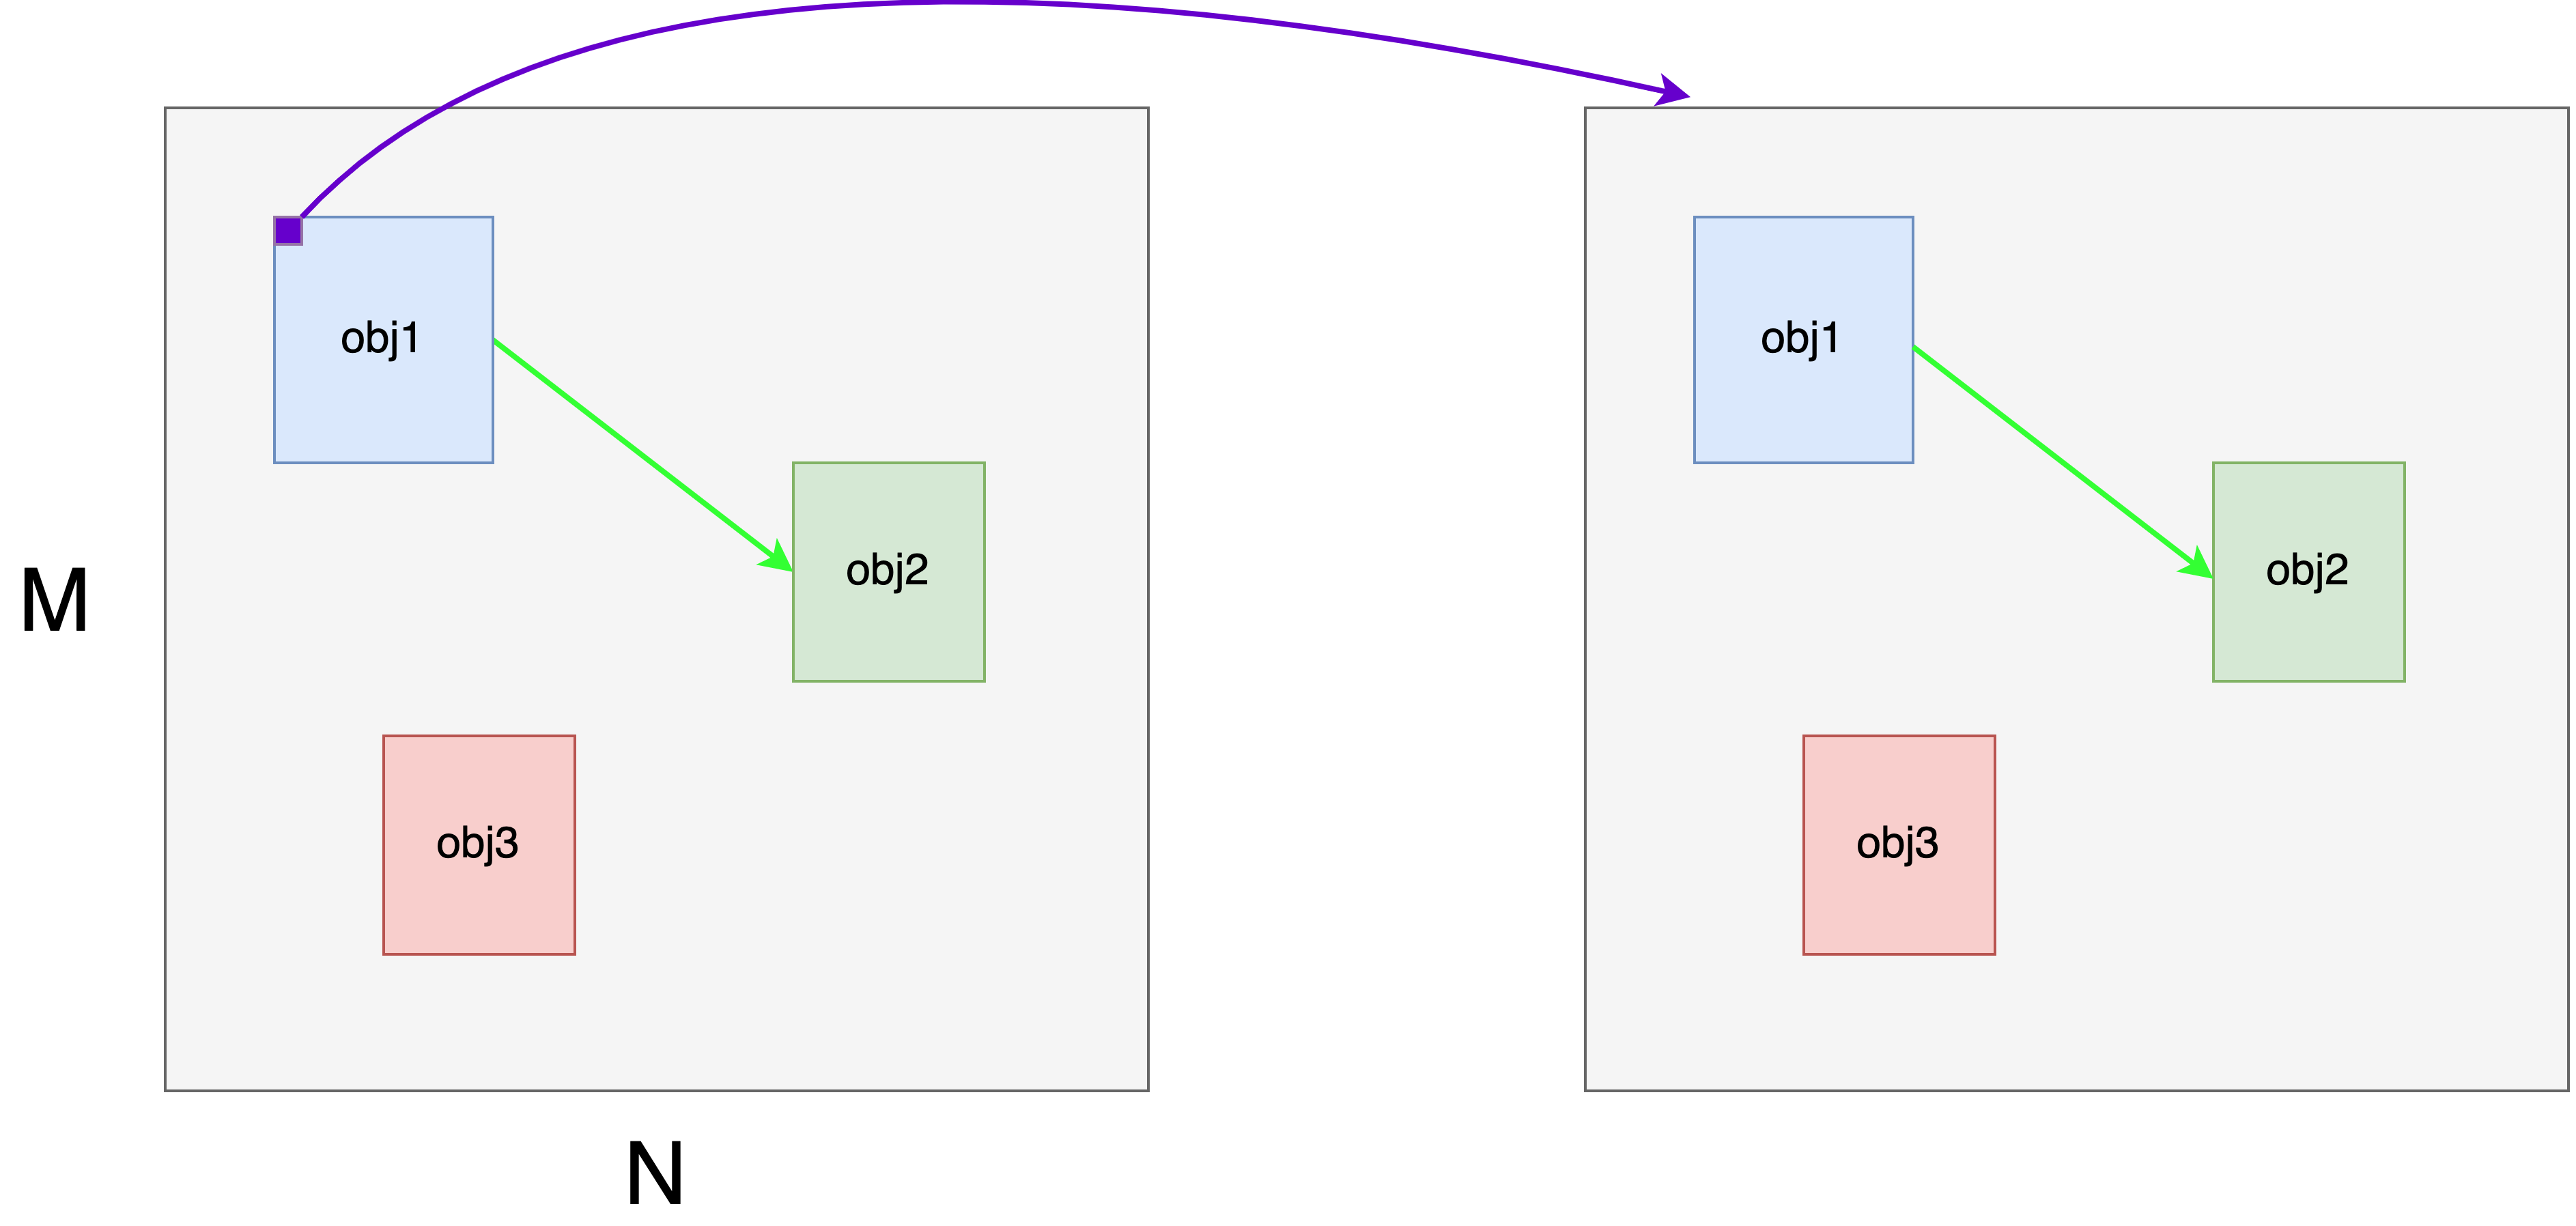
\includegraphics[width=0.8\linewidth]{figures/pixel_attention_idea}
			\label{fig:idea_pixelloss_a}
	\end{minipage}}
	
	\subfigure[The relationship between objects.]{
		\begin{minipage}[t]{7cm}
			\centering
			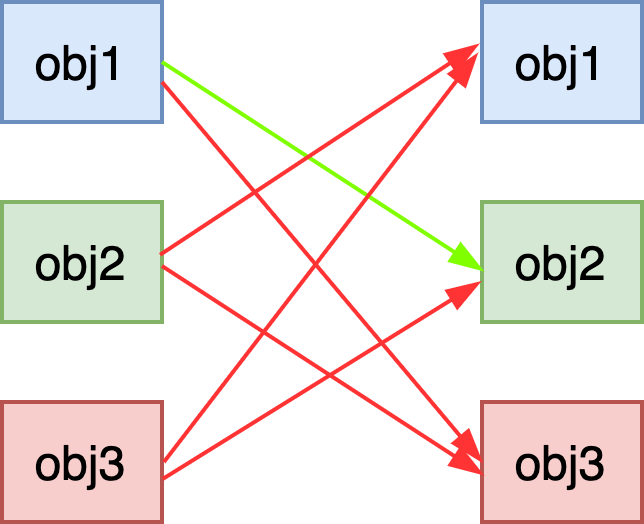
\includegraphics[width=0.8\linewidth]{figures/pixel_relation}
			\label{fig:idea_pixelloss_b}
	\end{minipage}}
	\subfigure[The attention map of each pixel of the image feature.]{
		\begin{minipage}[t]{7cm}
			\centering
			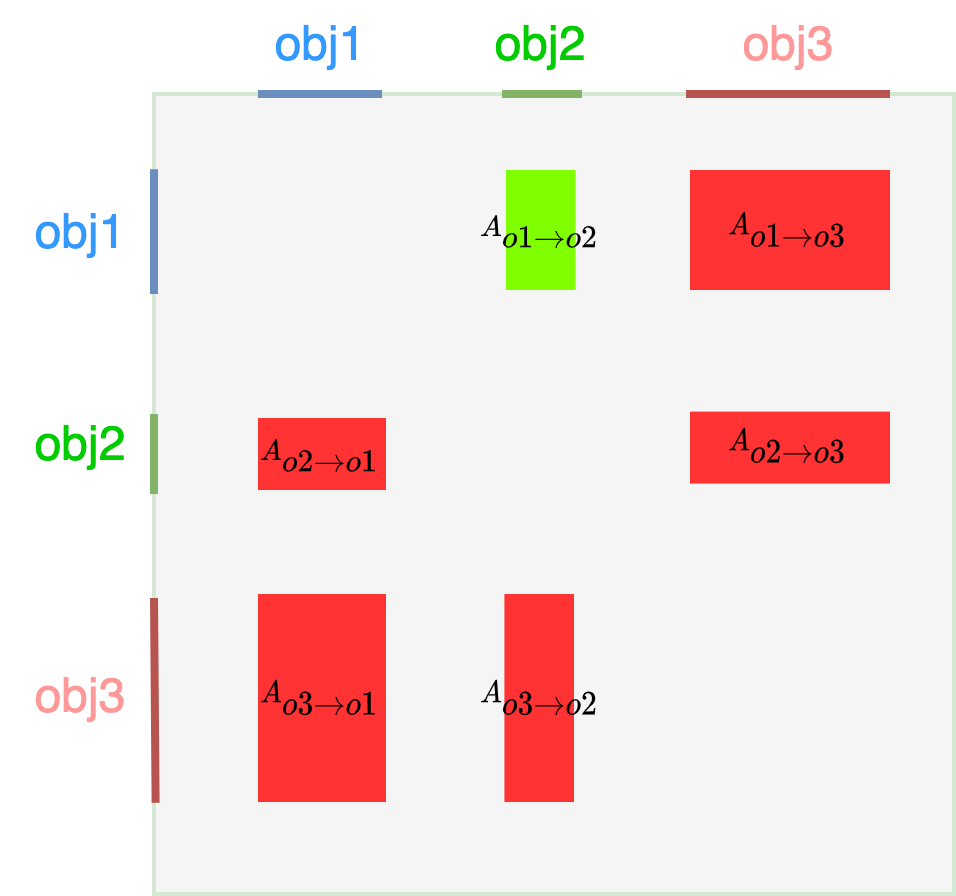
\includegraphics[width=0.9\linewidth]{figures/pixel_attentionmap}
			\label{fig:idea_pixelloss_c}
	\end{minipage}}
	\caption[The idea of the pixel-based attention]{The idea of the pixel-based attention. The Fig.(a) shows, that the first pixel of $object_1$ performs operations on all pixels to get its attention weights of the entire image. The Fig.(b) shows, that there is only relationship between $object_1$ and $object_2$ (the green line), there are no relationship between the others(the red line). The Fig.(c) show the position of the attention weights of  relation pairs. The green box represents a relationship, the red boxes means no relationship.}
	\label{fig:idea_pixelloss}
\end{figure}


\subsection{Idea of Pixel-based attention}
\label{sec:pixelbaseatt}
We perform multi-head self-attention operation on a down-sampled feature map. According to the Equation~\ref{equ:self_attention},  the attention weights between each pixel in the down-sampled image feature are computed. As shown in Fig.~\ref{fig:idea_pixelloss_a}, the size of down-sampling feature map is $  M\times N $, so an attention map with a size of $ (MN)^2 $ is obtained. Take the first pixel in $ object_1 $ as an example: when manipulating self attention, this pixel performs operations on all pixels to get its attention weights of the entire image, which are displayed as a line in the attention map, as shown in the blue line in Fig.~\ref{fig:idea_pixelloss_c}. These attention weights are represented as:
$$ \forall Attention_{p^1_{obj_1} \to p^i_{img}} , p^i_{img} \in \mathbb{P}_{img} $$ $ p^1_{obj_1} $ is the first pixel in $ object_1 $, and $ p^i_{img} $ is the $ i^{th} $ pixel in down-sampled feature map, and $ \mathbb{P}_{img} $ is the set of pixels in the down-sampled feature map. According to this blue line, the attention of the first pixel in $ object_1 $ to all pixels in $ object_2 $ can be observed, which is represented as the intersection of the blue line and the green box in the figure.

This attention map can be used to determine whether there is a relationship between $ object_1 $ and $ object_2 $, so the attention of each pixel in $ object_1 $ to all pixels in $ object_2 $ should be studied, which is $$ \forall Attention_{p^i_{obj_1} \to p^j_{obj_2}} , p^i_{obj_1} \in \mathbb{P}_{obj_1}, p^j_{obj_2} \in \mathbb{P}_{obj_2}  $$ and it is shown as the green box in the Fig.~\ref{fig:idea_pixelloss_c}, $ \mathbb{P}_{obj_i} $is defined as the pixel set of $ object_i $. In this figure, there are also red boxes, which indicates that there is no relationship between the corresponding objects. For example, the red box $ B2 $ means that $ object_1 $ has no relationship with $ object_3 $.

The main idea of Pixel-base attention is to judge whether there is a relationship between $ object_m $ and $ object_n $ through the attention map. As shown in Fig.~\ref{fig:idea_pixelloss_c}, the color of the boxes reflect whether there is a relationship between objects, and the color may be determined by attention weights in the experiment, the attention weights of the green box should be higher than the red one.

\begin{figure}[H]
	\centering
	\subfigure[No relation between \textit{roof} and \textit{tree}.]{
		\begin{minipage}[t]{6cm}
			\centering
			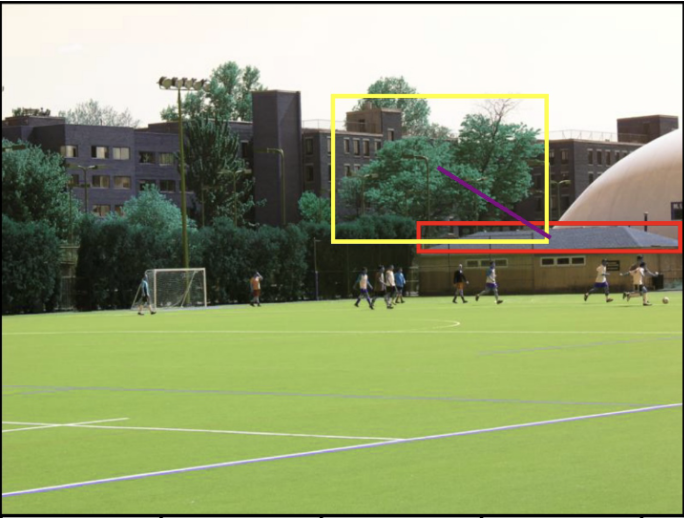
\includegraphics[width=1\linewidth]{figures/roof/img1}
	\end{minipage}}
	\subfigure[$ \forall Attention_{p^i_{roof} \to p^j_{tree}}  $'s position.]{
		\begin{minipage}[t]{6cm}
			\centering
			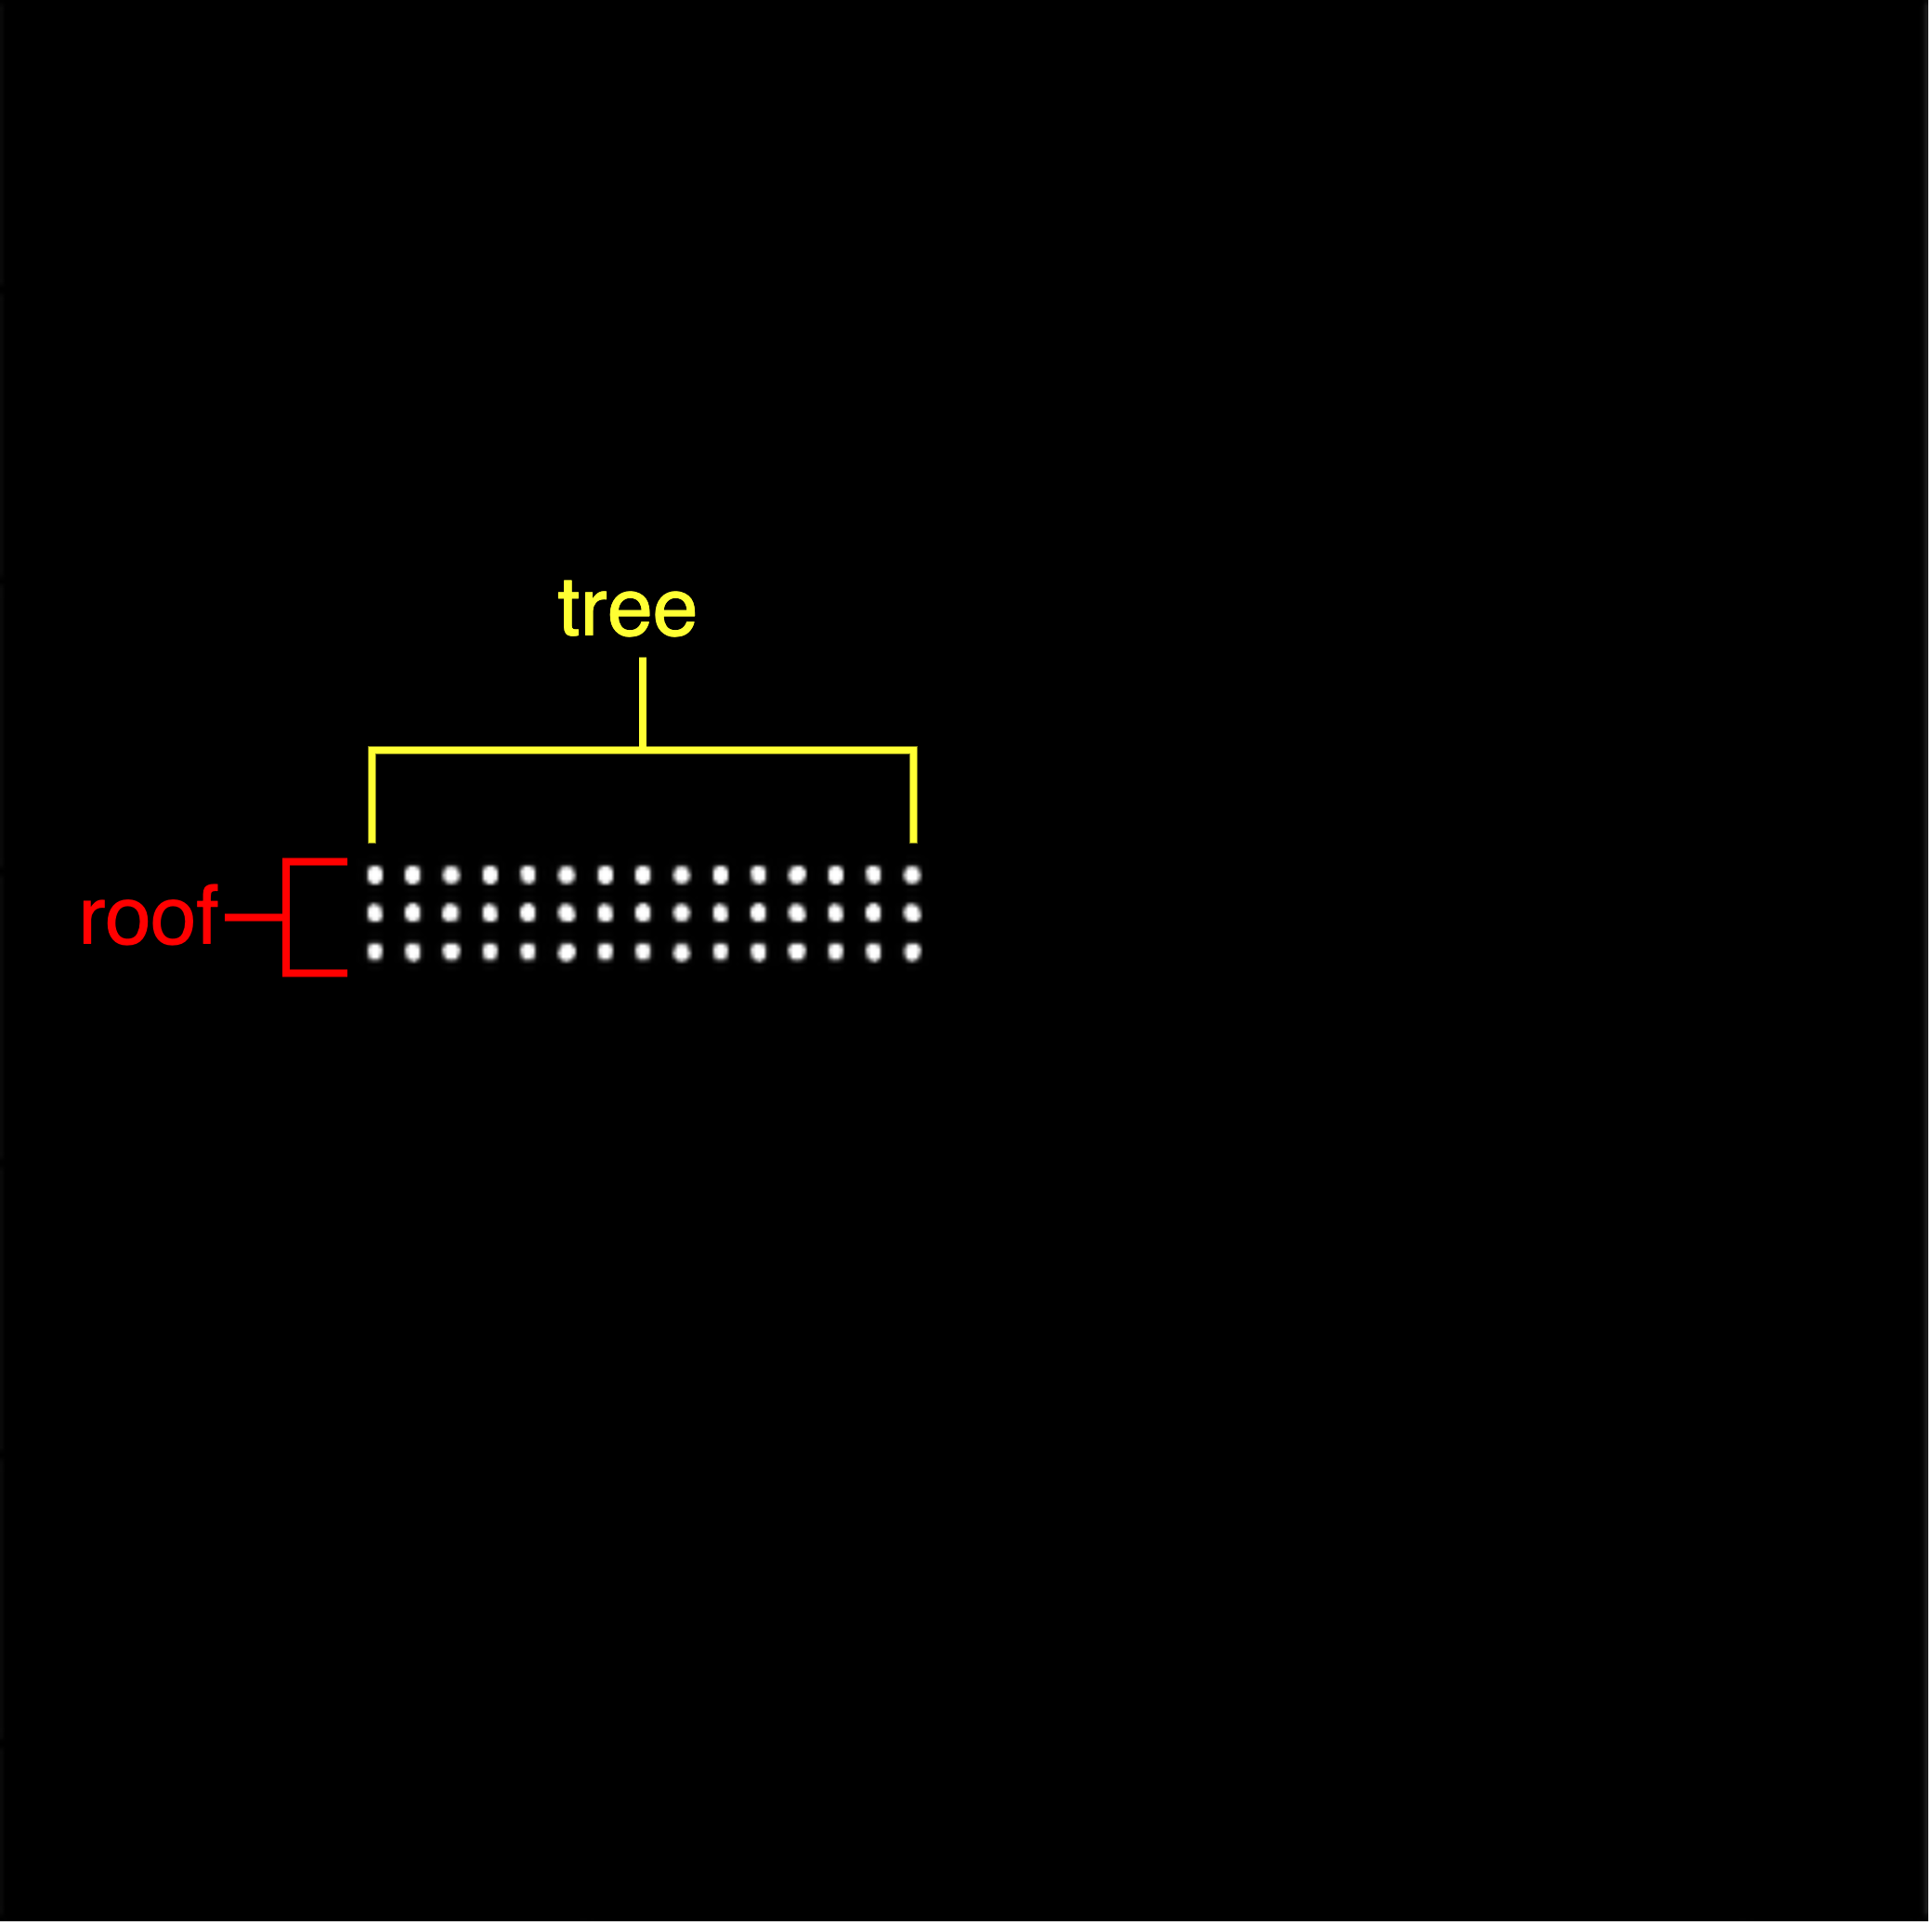
\includegraphics[width=0.8\linewidth]{figures/roof/map1}
	\end{minipage}}
	
	\subfigure[Ground truth relation: \textit{roof on building}.]{
		\begin{minipage}[t]{6cm}
			\centering
			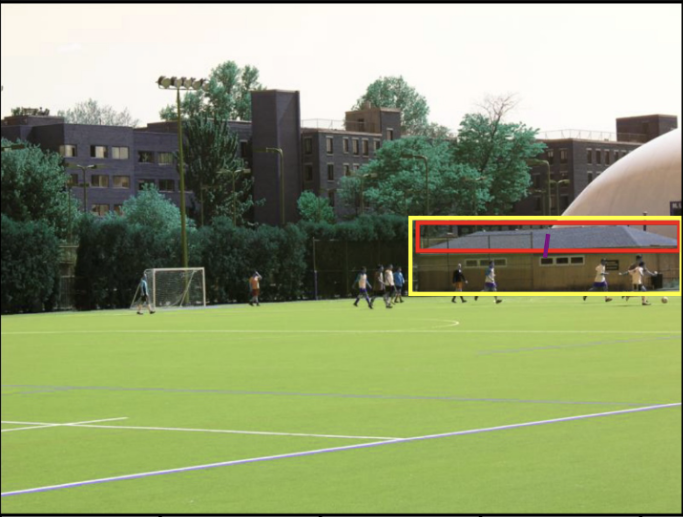
\includegraphics[width=1\linewidth]{figures/roof/img2}
	\end{minipage}}
	\subfigure[ $ \forall Attention_{p^i_{roof} \to p^j_{building}}  $'s position.]{
		\begin{minipage}[t]{6cm}
			\centering
			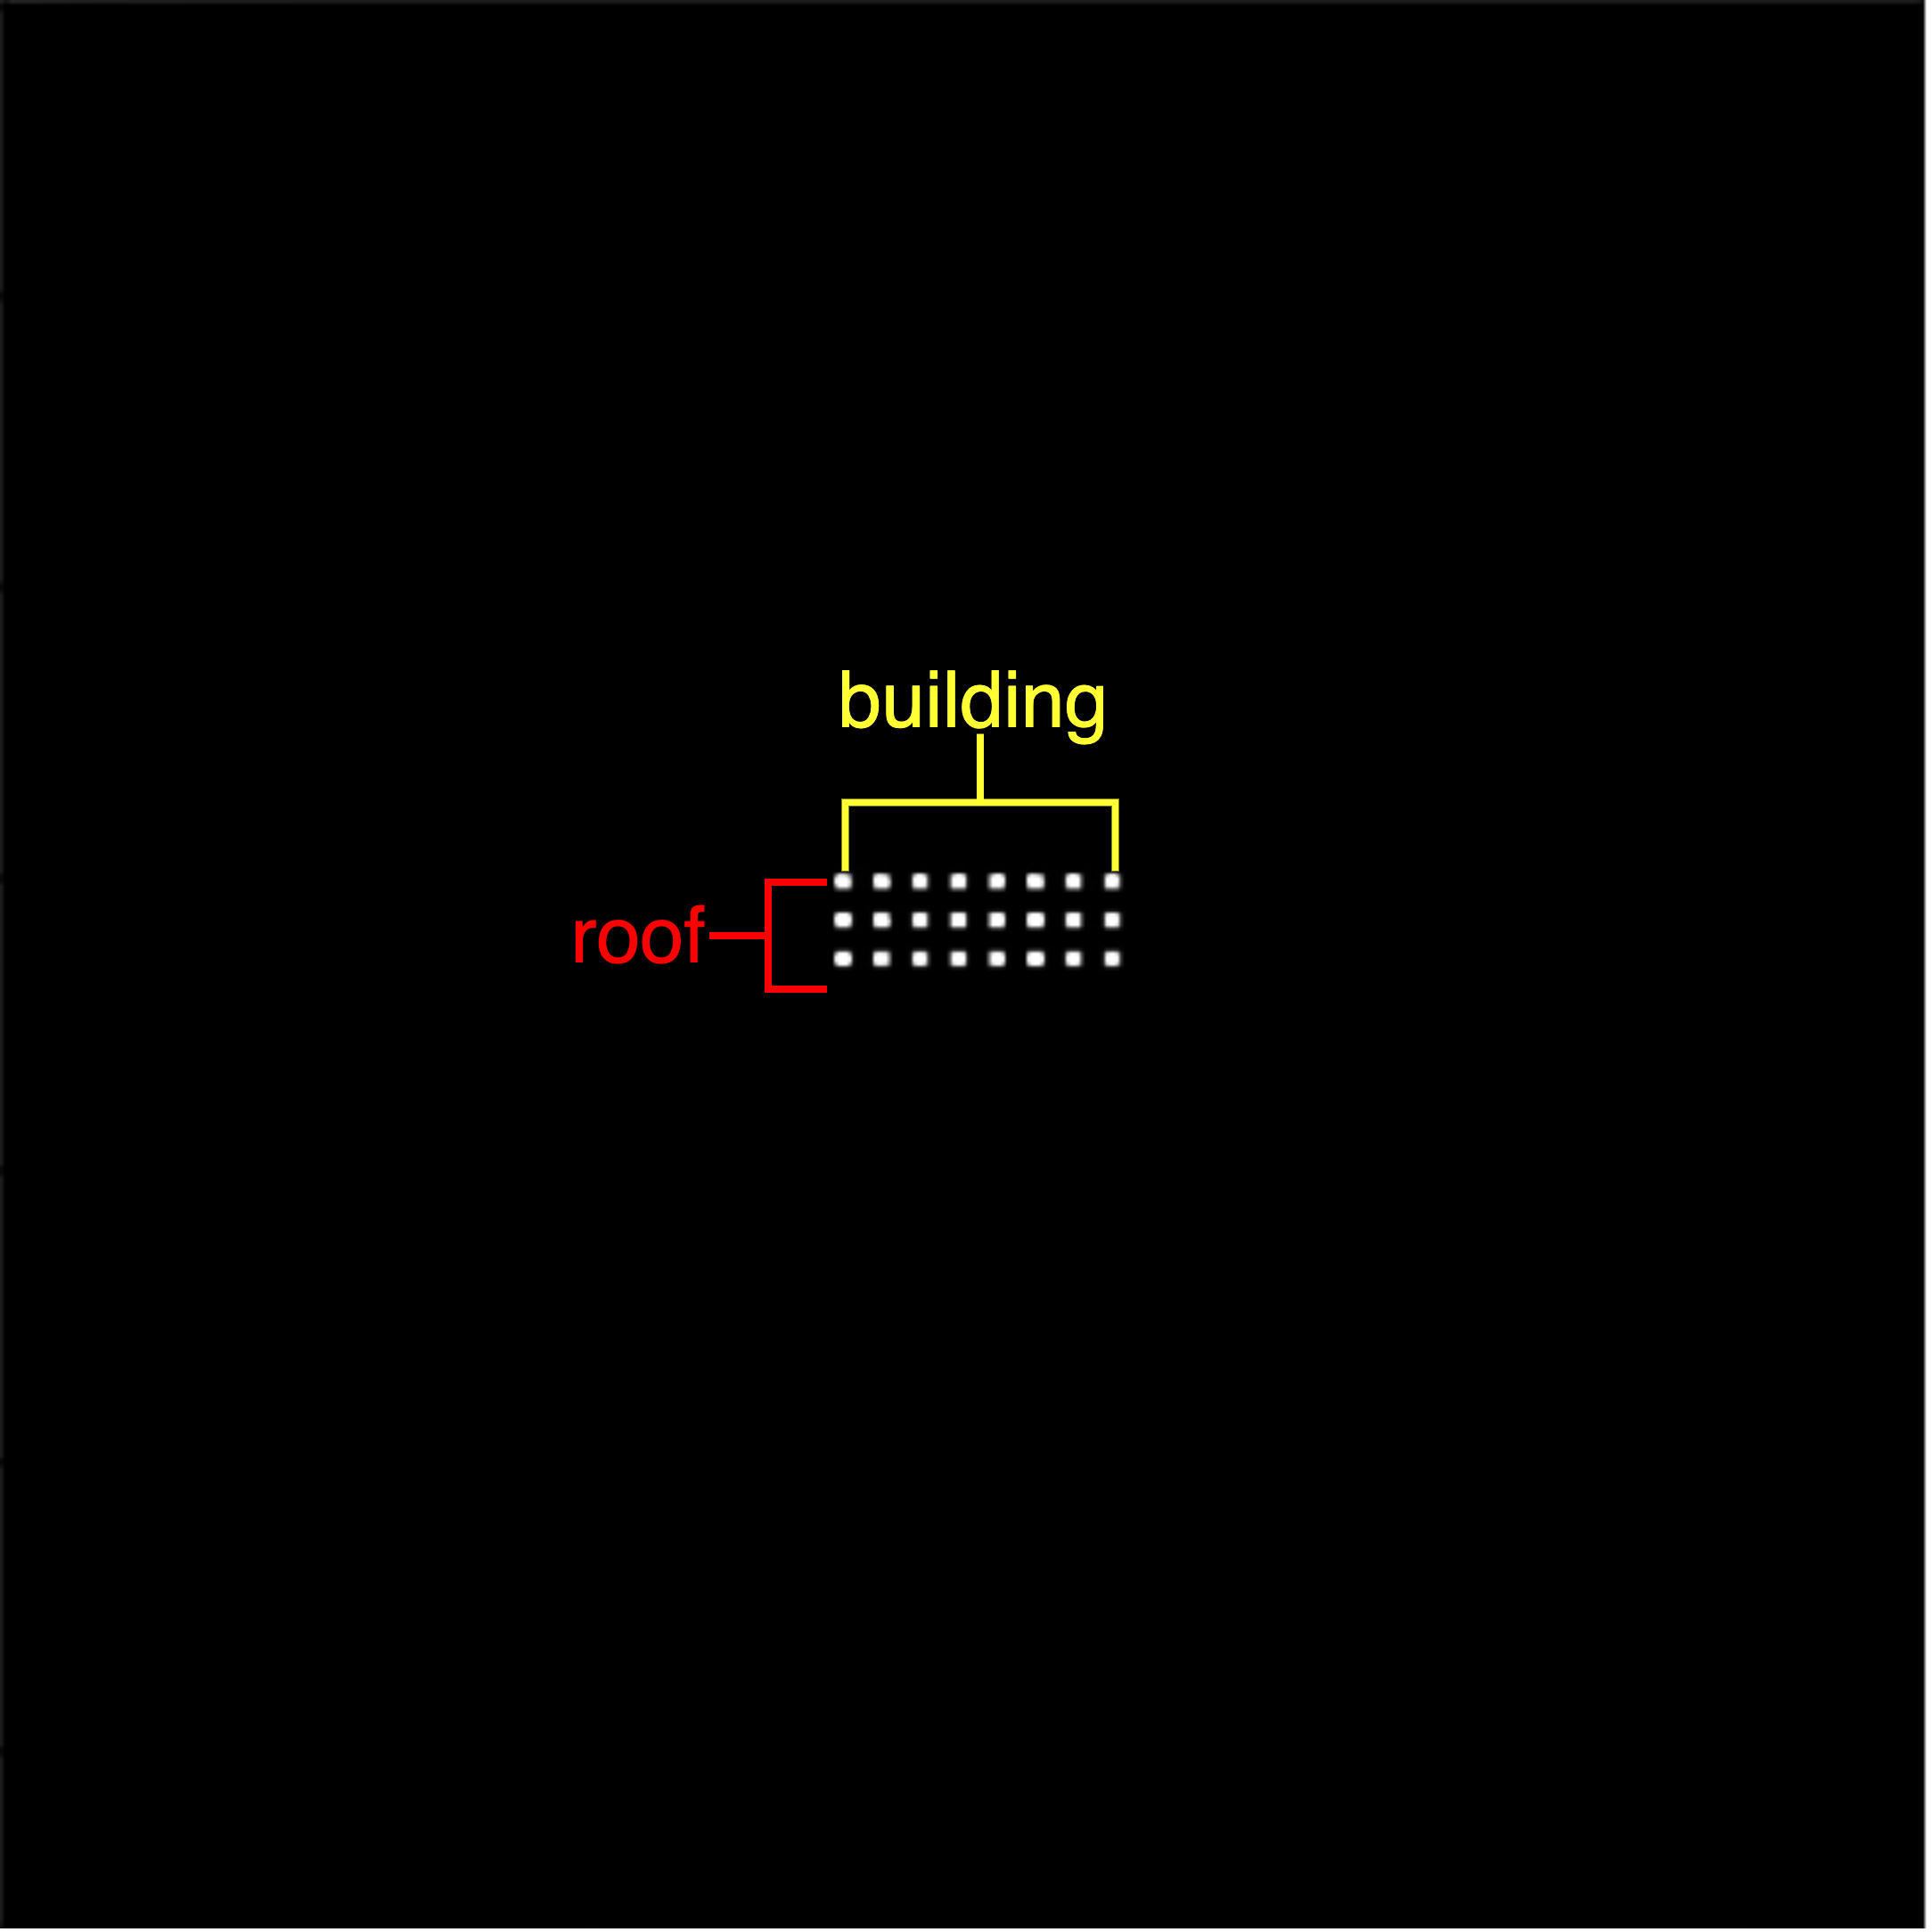
\includegraphics[width=0.8\linewidth]{figures/roof/map2}
	\end{minipage}}
	
	\caption[An example of Pixel-based attention]{Relation pair in image and its position on attention map.}
	\label{fig:ideamethod1}
\end{figure}

Figure~\ref{fig:ideamethod1} shows the position of the attention in a real picture. The sub-figure(a) shows that when the subject is \textit{tree} and the object is \textit{roof}, there is no relationship between them, and the position of $ \forall Attention_{p^i_{roof} \to p^j_{tree}}  $ in the attention map is represented as the white area in sub-figure(b). Similarly, the sub-figure(c) represents a ground truth relation: \textit{roof on building}, and the position of $ \forall Attention_{p^i_{roof} \to p^j_{building}}  $ in the attention map is the white area in the sub-figure(d). The attention weights of the white area in sub-figure(b) are expected much lower than other areas, or even equal to 0, which indicates that there is no relationship between the object \textit{roof} and the object \textit{tree}.The attention weights of the white area in sub-figure(d) are much higher than other areas, so the relationship between $ roof $ and $ building $ exits. This attention map should be able to show that each pixel in the $ roof $ can focus on all the pixels in the $ building $ instead of all the pixels in the $ tree $.

%There are three objects in the picture, of which only object1 and object2 have a relationship.
%Assuming that in Figure~\ref{fig:ideamethod1} we obtained the down-sampled image feature size of 512x66x50 through the backbone, that is, each layer od the feature has 3300 pixels, we convert it into a sequence of 3300x512, then input it into the Multihead Self-Attention module, and get an attention map size of 3300x3300 . We look for the pixel of the subject in the row of the attention map, and look for the pixel of the object in the column of the attention map ,to find the attention weight between the subject and object pixels. Eg. the ground truth pair $ \left\langle roof, building \right \rangle $ in Figure~\ref{fig:ideamethod1} is located in the attention map as shown in the lower right corner of Figure ~\ref{fig:ideamethod1}.



We hope that through the training of our model, the attention weight of ground truth pairs can be higher than those of pairs without relation. In this way, we can use the attention weight in the evaluation to determine which pairs are most likely to be related.


\subsection{ Implementation of Pixel-based Attention}
As shown in following Figure~\ref{fig:method1baseline}, first enter an image into the  backbone VGG16~\cite{simonyan2015deep}(see Figure~\ref{fig:vgg16}.) to obtain a down-sampled image feature \textit{feature},  then the \textit{feature} is passed through a multi-head self-attention module to generate an attention map and a new image feature \textit{feature2}. Finally, the features of the subject, predicate and object are extracted by ROI Align (see  Sec.~\ref{fig:roialign}), and sent to the predicate classifier as input.


\begin{figure}[H]
	\centering
	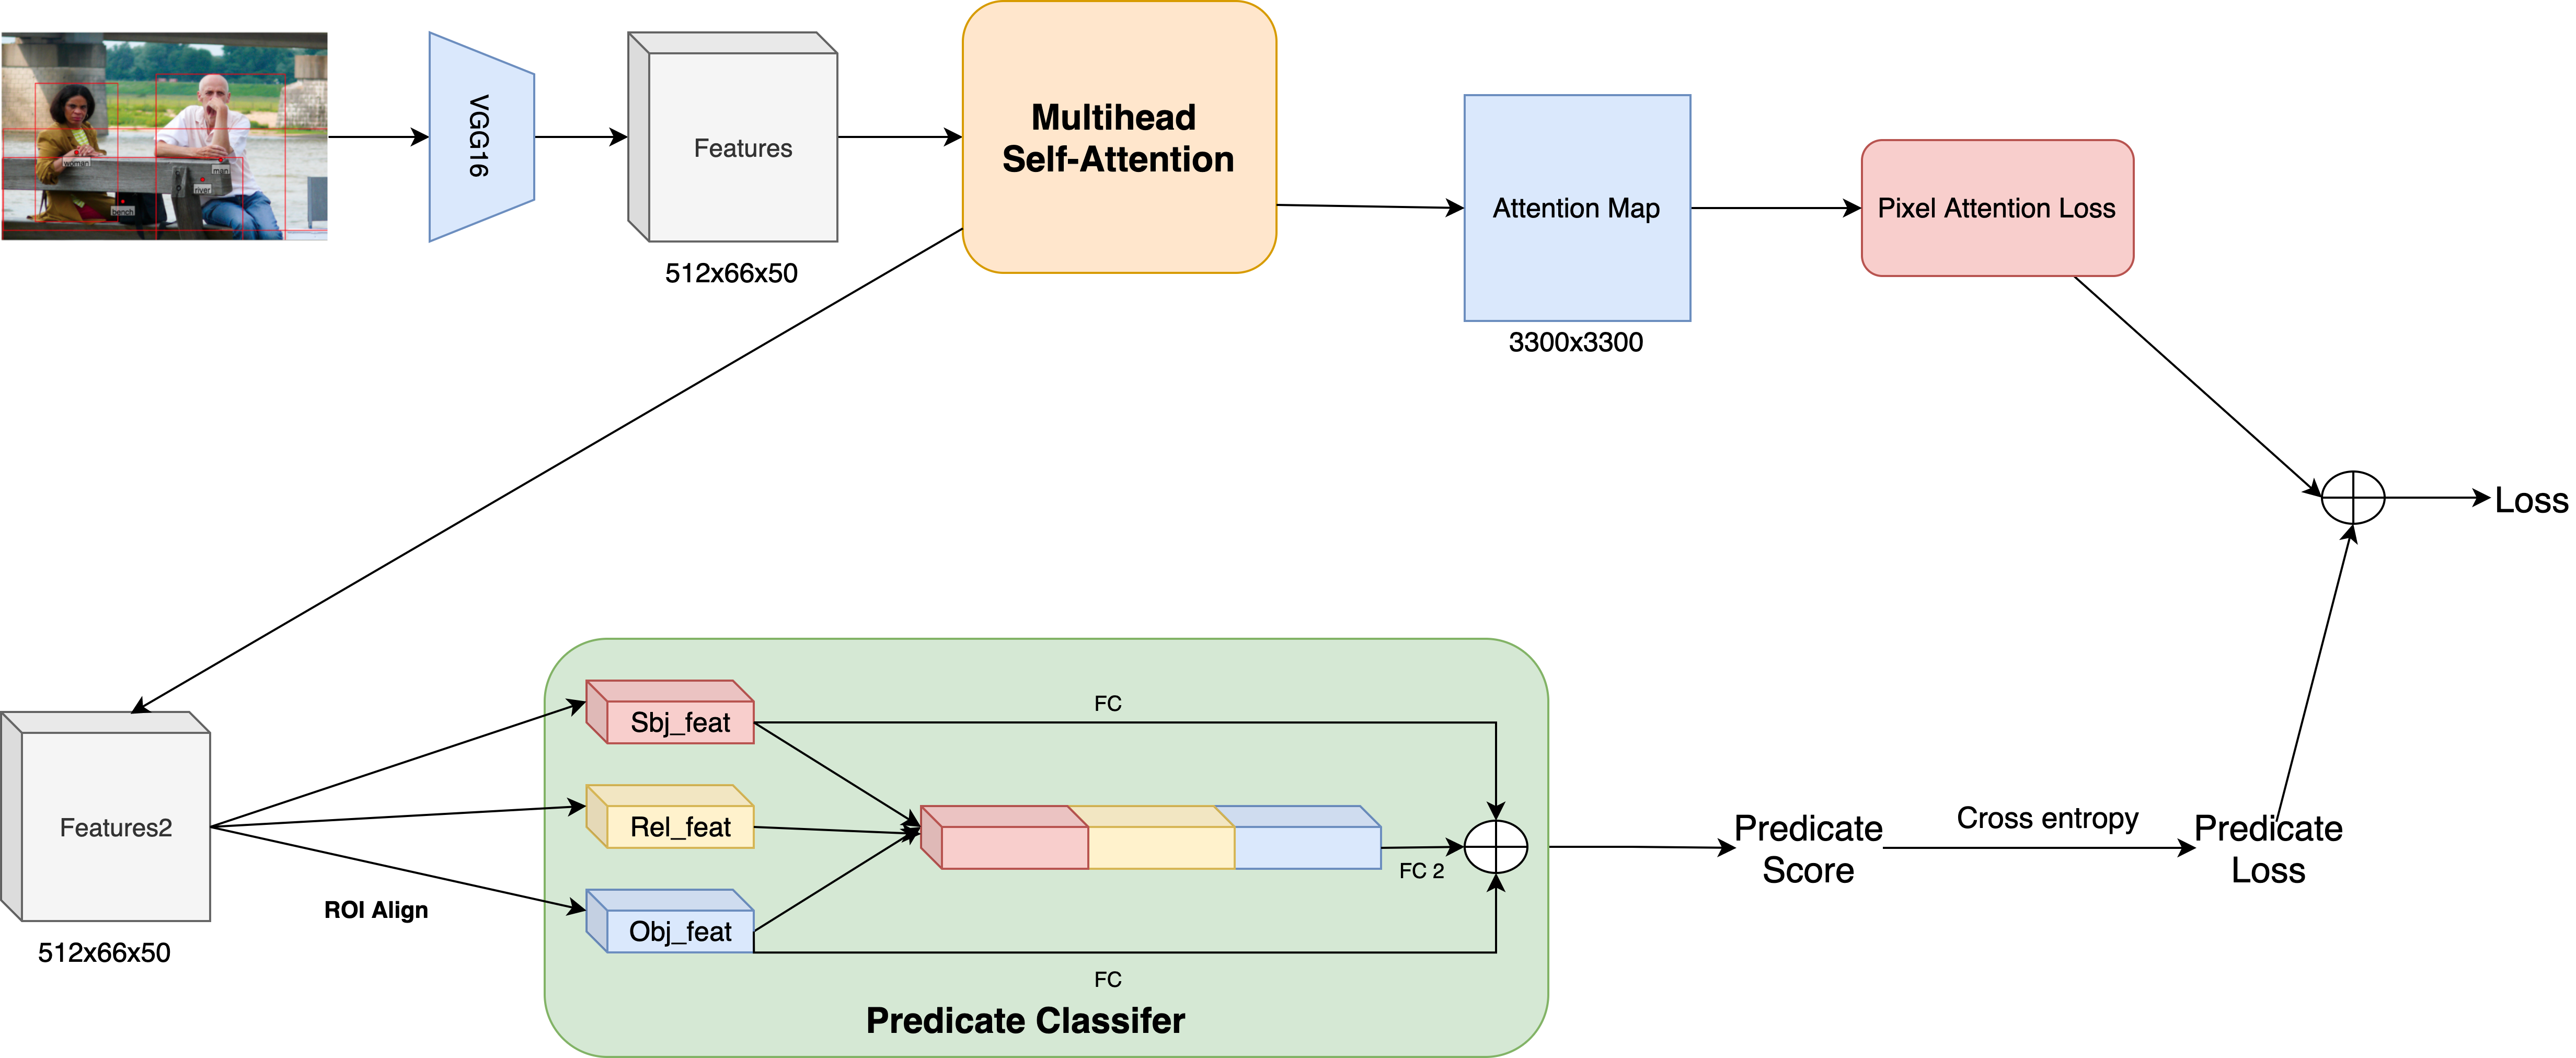
\includegraphics[width=1\linewidth]{figures/method1_baseline}
	\caption[The baseline of the first method: Pixel-based attention]{The baseline of the  first method: Pixel-based attention}
	\label{fig:method1baseline}
\end{figure}

\subsection{Pixel  Attention Loss}
\label{sec:pixelattentionloss}
As mentioned above, the main idea of pixel-based attention is to compute the attention weights between a subject's pixels and all objects' pixels in a pixel-to-pixel attention map, then the object that has the most relevant to the subject can be found. Therefore, the pixel attention loss function is designed to focus the subject on its most relevant objects.

In Fig.~\ref{fig:idea_pixelloss_c}, there are 3 objects and 6 relation pairs between them, so the attention weights of 6 regions in the attention map should be paid more attention to, of which only the attention weights in the green box are represented as ground truth relations. So the loss function needs to increase the attention weights of the green boxes and decrease the attention weights of the red boxes. Ranking loss(see in Sec.~\ref{sec:rankingloss}) is more suitable to complete this work, wherefore we designed the following loss function:
\begin{equation}\label{pixel_attention_loss}
	loss_{attention}=max(0, \frac{1}{m}\sum_{m}Att_j^{no\_rel}-\frac{1}{n}\sum_{n}Att_i^{rel}+0.25
	/3300)
\end{equation}

where:
\begin{itemize}
	\item $ Att_j^{no\_rel} $ : the $ j^{th} $ attention weight of no-relation pairs.
	\item $ Att_i^{rel} $ :  the $ i^{th} $ attention weight of ground truth relation pairs.
	\item Margin=0.25/3300.
	\item m: the sum of $ Att_j^{no\_rel}$.
	\item n: the sum of $ Att_i^{rel} $.
\end{itemize}


For the example in Fig.~\ref{fig:idea_pixelloss_c}, it can be expressed as:
\begin{align*}
	Att_j^{no\_rel} \in & \forall Attention_{p^k_{obj_1} \to p^j_{obj_3}}  \cup \   \forall Attention_{p^k_{obj_2} \to p^j_{obj_1}} \cup \\ 
	& \forall Attention_{p^k_{obj_2} \to p^j_{obj_3}} \cup \ \forall Attention_{p^k_{obj_3} \to p^j_{obj_1}} \cup \\ 
	& \forall Attention_{p^k_{obj_3} \to p^j_{obj_2}}
\end{align*}

\begin{equation*}
	Att_i^{rel} \in  \forall Attention_{p^k_{obj_1} \to p^j_{obj_2}} 
\end{equation*}

To adjust the values of $ \forall Att_j^{no\_rel}  $ and the values of $ \forall Att_i^{rel} $ , the loss function is applied. Specifically, the values of $ \forall Att_j^{no\_rel}  $ become lower, and the values of $ \forall Att_i^{rel} $ become higher. And in this thesis, the mean value of them are used. Whether there is a relationship can be judged through the attention value of each pair during evaluation.

Although the pixel attention is potential to indicate that whether there is the interaction between two objects, or more accurately, two regions, we discover some drawbacks in the experiments (see Sec.~\ref{sec:experimentpixel}). When there is overlap between $ \forall Att_j^{no\_rel}  $ and $ \forall Att_i^{rel} $, obviously our loss function does not play any role in training, and the same is true in experiments, almost every figure has overlap between them.
So finally we change the method from pixel-based to box-base, and a complete transformer structure is introduced. Our final model Retina Net is shown in the next section.
%We have studied the attention map, and its meaning is the attention between all pixels of the image feature( $ Attention_{p_i\to p_j}, \  wehre \quad p_i,p_j\in \mathbb{P}_{img} $) , $ \mathbb{P}_{img}  $is a collection containing all pixels of the image feature from VGG16.
%
%We want to know whether $ obj_i  $has a relationship with $ obj_j$ through attention. For example, we have three objects ($ obj_1 $, $ obj_2 $, $ obj_3 $) . Assuming there is a relationship between $ obj_1 $ and $ obj_2 $, $ obj_1 $ and $ obj_3 $, $ obj_2 $ and $ obj_3 $ are not related, see in Fig.~\ref{fig:idea_pixelloss_a}, the green line means $ pair <obj_1,obj_2> $ has relationship, while the red line means the other pairs have no relationship. 
%
%We first have the following definition: 
%$$ Attention_{p_{obj_i}\to p_{obj_j}},\ where \quad p_{obj_i} \in \mathbb{P}_{obj_i},\  p_{obj_j} \in \mathbb{P}_{obj_j} $$
%Where $ \mathbb{P}_{obj_i}, $ represents the collection of all pixels of $ obj_i $ on the image feature obtained from VGG16. $  Attention_{p_{obj_i}\to p_{obj_j}} $ means the attention weight between the pixel $ p_{obj_i} $ and the pixel $ p_{obj_j} $. In Fig.~\ref{fig:idea_pixelloss_b} we abbreviate it as $ A_{oi \to oj} $. and we can see the green area means there is a relationship.
%
%
%
%we want to know which pair is more relevant in evaluation through the attention weights between each pixel on the down-sampled image feature, thus we design a pixel attention loss as following:
%\begin{equation}\label{pixel_attention_loss}
%	loss_{attention}=max(0, \frac{1}{m}\sum_{m}Att_j^{no\_rel}-\frac{1}{n}\sum_{n}Att_i^{rel}+0.25
%	/3300)
%\end{equation}
%
%Where:
%
%\begin{itemize}
%	\item $ Att_j^{no\_rel} $ : the attention weight of the pixel j of no-relation pairs.
%	\item $ Att_i^{rel} $ :  the attention weight of the pixel i of gt relation pairs.
%	\item Margin=0.25/3300 is quarter the average of the attention map.
%\end{itemize}
%
%
%\begin{align*}
%	Att_j^{no\_rel} \in & \forall Attention_{p^k_{obj_1} \to p^j_{obj_3}}  \cup \   \forall Attention_{p^k_{obj_2} \to p^j_{obj_1}} \cup \\ 
%	& \forall Attention_{p^k_{obj_2} \to p^j_{obj_3}} \cup \ \forall Attention_{p^k_{obj_3} \to p^j_{obj_1}} \cup \\ 
%	& \forall Attention_{p^k_{obj_3} \to p^j_{obj_2}}
%\end{align*}
%
%\begin{equation*}
%	Att_i^{rel} \in  \forall Attention_{p^k_{obj_1} \to p^j_{obj_2}} 
%\end{equation*}

%For example, in Fig.~\ref{fig:idea_pixelloss_b} , our $Att_i^{rel} $  is $ A_{o1 \to o_2} $ (the green area) and  the $ Att_j^{no\_rel} $ are $ A_{o1 \to o_3}  $,  $ A_{o2 \to o_1}  $, $ A_{o2 \to o_3}  $, $ A_{o3 \to o_1}  $ and $ A_{o3\to o_2}  $(the red areas). We use our attention loss to make attention weights of the green area in this figure higher and the value of the red area lower. In this way, we can judge which can have a relationship through the attention value of each pair during evaluation.

%For this method, we have conducted many attempts and experiments. Through our experimental verification, we found that the results did not achieve our expectations. After thinking, we found a very serious problem. For the specific experimental results and analysis, please refer to the following chapters. So we changed our thinking, changed from pixel-based to box-based, and used the complete transformer encoder decoder structure, and added our own design here. Next we will introduce our final model Retina Net.

\section{Retina Net}
\label{sec:retinanet}
Inspired by pixel-based attention, we propose a new transformer-based model structure Retina Net. It uses box-wise attention to obtain the global context and avoids the overlap between pixels in the relation pair. It performs well in the three different evaluation methods of VRD. For these three evaluation methods, we have also done different Model optimization.

In the framework (see Fig.~\ref{fig:my_model}), we propose a new visual relationship detection network. A convolutional neural network (CNN) backbone and an \textit{Encoder} module generate visual features of the images. A \textit{Object Decoder} module is to obtain object features and  the context between each entity, and a \textit{Relation Decoder} module is to obtain the context between entities and relations, finally a \textit{Predicate Classifer} module is applied to predict predicates.

\begin{figure}[!htbp]
	\centering
	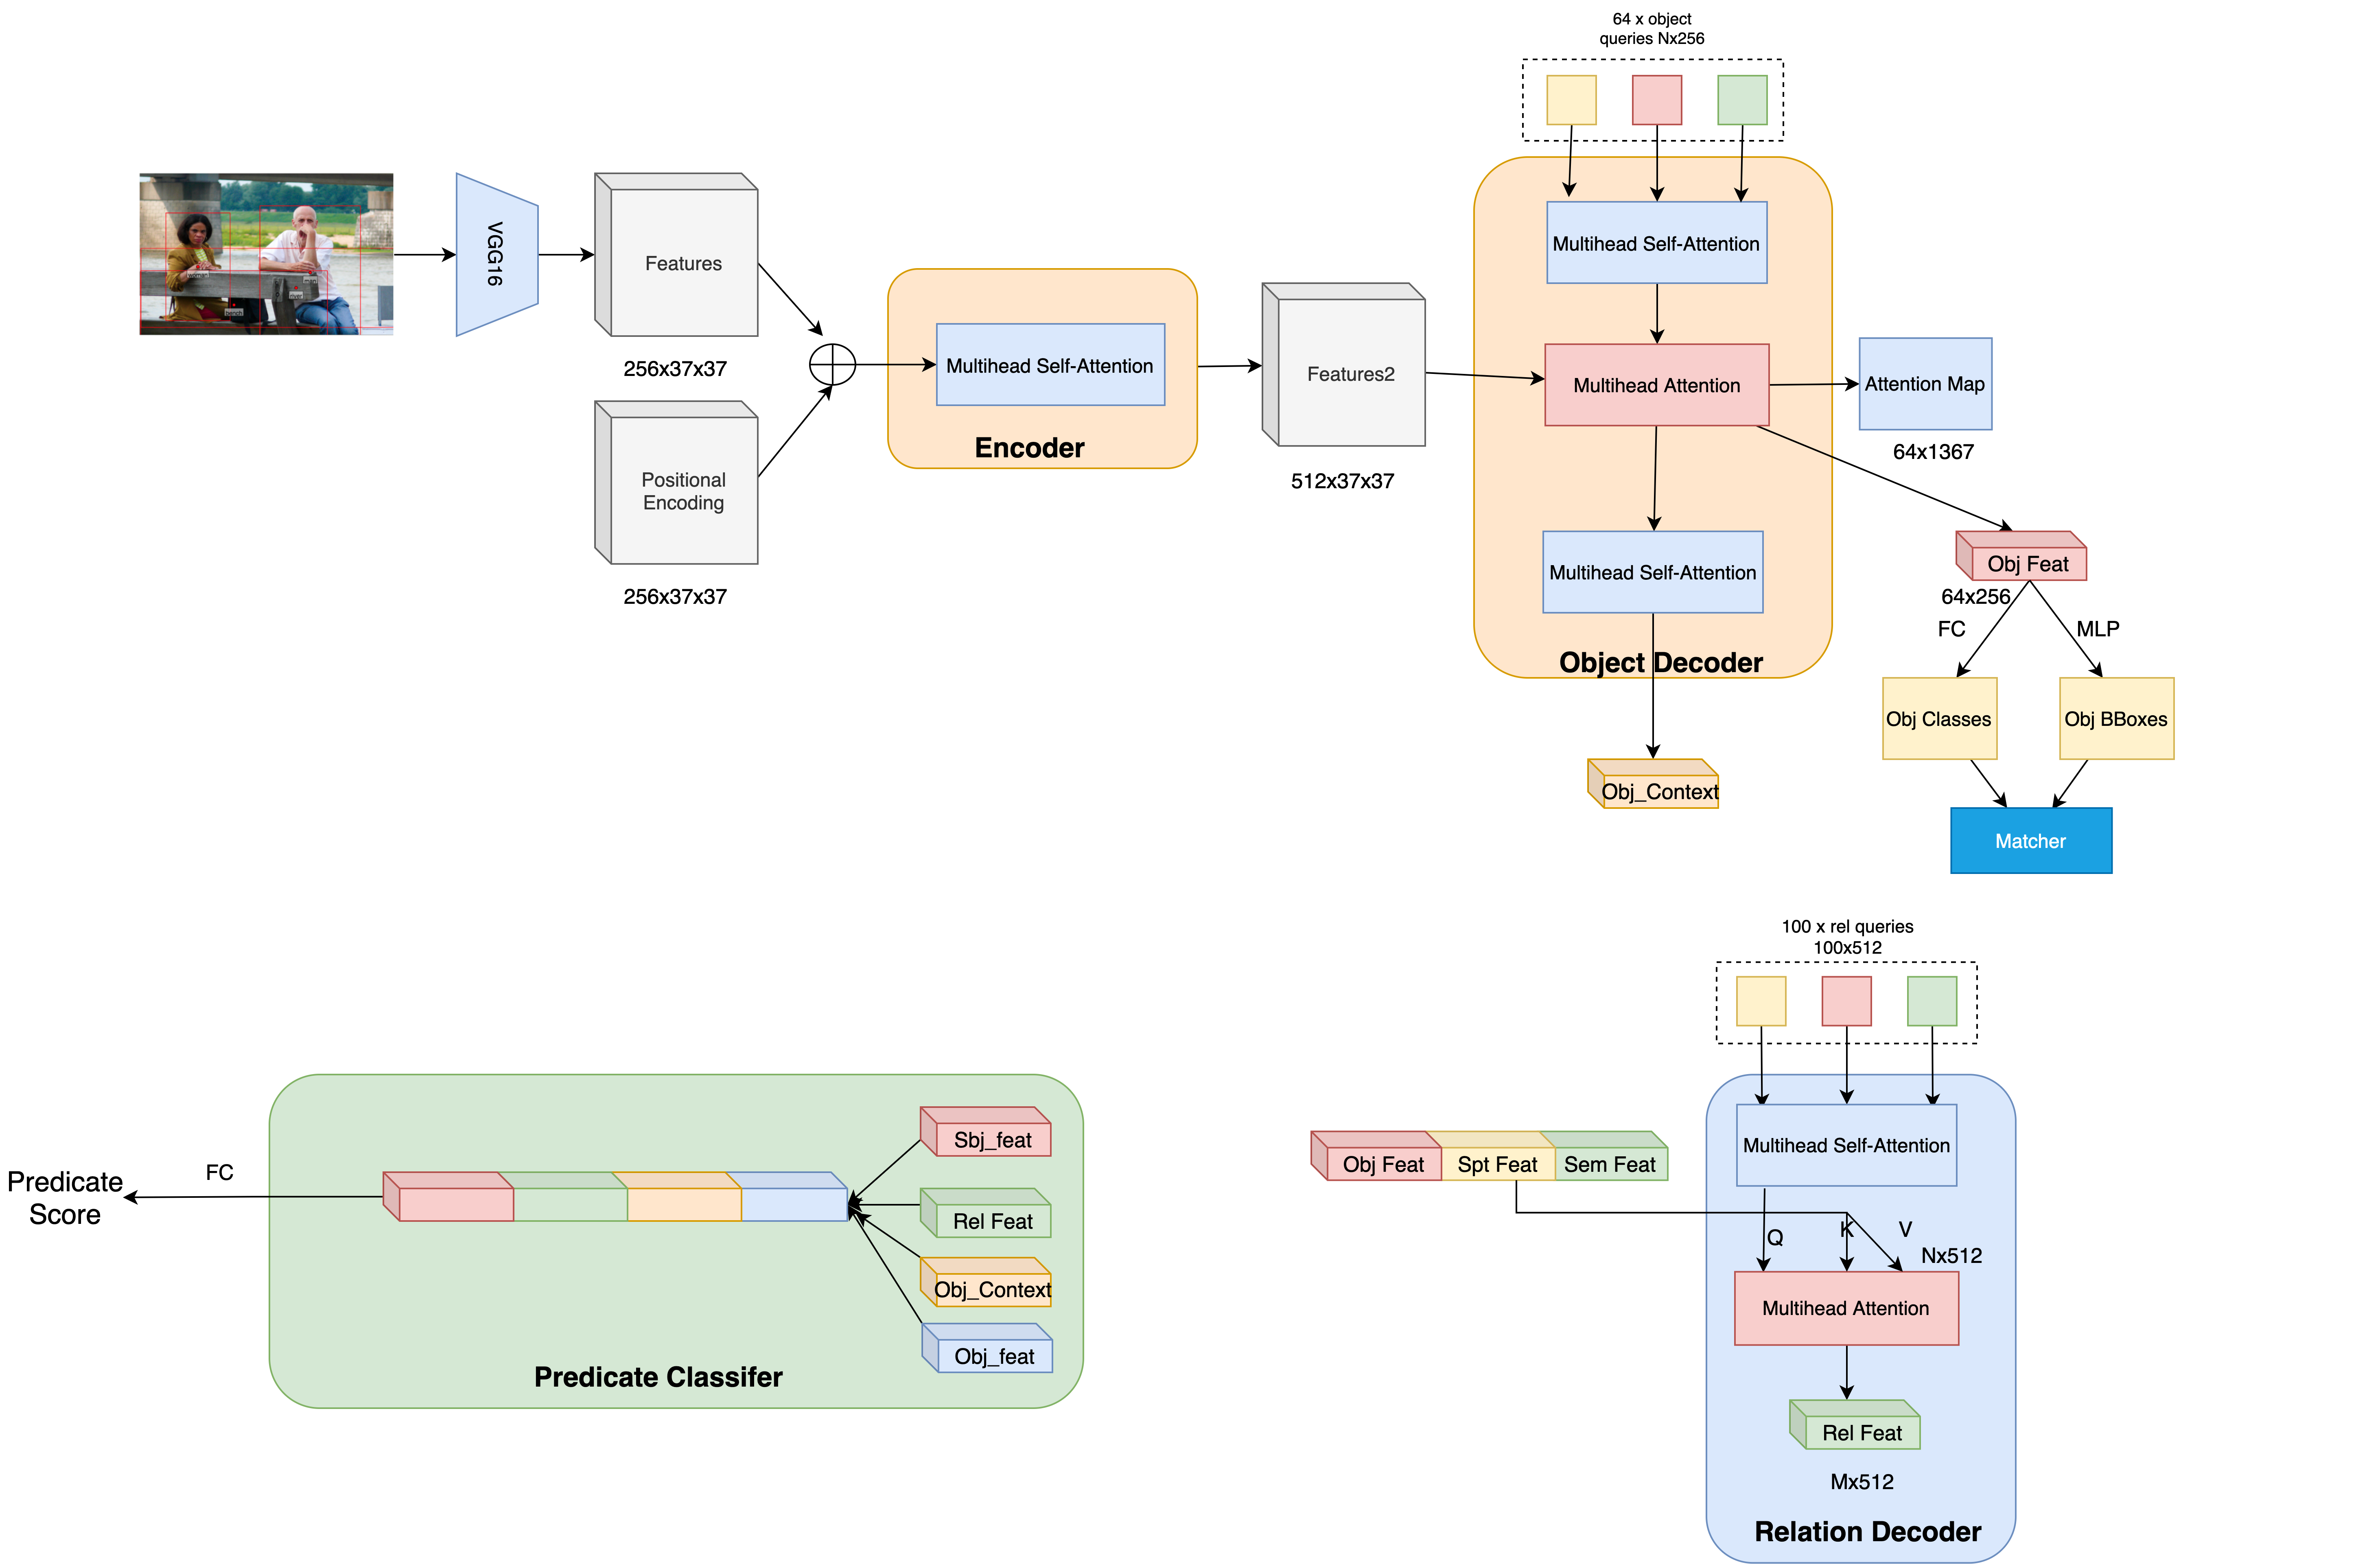
\includegraphics[width = 1\textwidth]{figures/my_model.png}
	\caption[The architecture of our model.]
	{The architecture of our model, which consists of a convolutional neural network (CNN) backbone, an Encoder, an Object Decoder, a Relation Decoder and a Predicate Classifier.}
	\label{fig:my_model}
\end{figure}

\label{sec:imagefeture}
\subsection{Generation of Image Feature Maps }

The first step is to extract the visual features from images by VGG16, and then the encoder performs self attention on the image features to obtain a pixel-wise visual feature(see Fig.~\ref{fig:imgfeatbaseline}).

In Figure ~\ref{fig:imgfeatbaseline} the image needs to be rescaled and padded to a uniform size of $ 3\times592\times592 $ before it is fed into the VGG16 backbone, and the scaled image is normalized with $ mean = [0.485, 0.456, 0.406 ]$ and $ std = [ 0.229, 0.224, 0.225]$. Then the basic visual feature $f^{vgg}_{img}$ of the image is extracted with VGG16, which has the size $512 \times 37 \times 37$. In order to reduce the amount of calculation, the feature will be compressed to a size $256 \times 37 \times 37$ through a convolutional layer, whose stride and kernel size are both 1. Subsequently,the $f^{vgg}_{img}$ of each layer is flattened  into a 1369x256 sequence signal. Since the encoder has no position information of the sequence signal in the image, it is necessary to introduce positional encoding to add position information to the sequence, and we use Equ.~\ref{equ:position_embedding} in this thesis. Finally, the image sequence feature with position code is fed to the multi-head self-attention module to compute a new image feature sequence with the same size, which can be reshaped to the image feature $f^{en}_{img}$ with the size of $256 \times 37 \times 37$.

In the above process, there are two image features, one is$f^{vgg}_{img}$ extracted through VGG16 and the other is $f^{en}_{img}$ obtained through encoder. They all contain the visual information of the image. The difference is that $f^{en}_{img}$ has piexl-wise interactive, which emphasizes which pixels will be paid more attention to and this is helpful for the object detection.


\begin{figure}[tbph!]
	\centering
	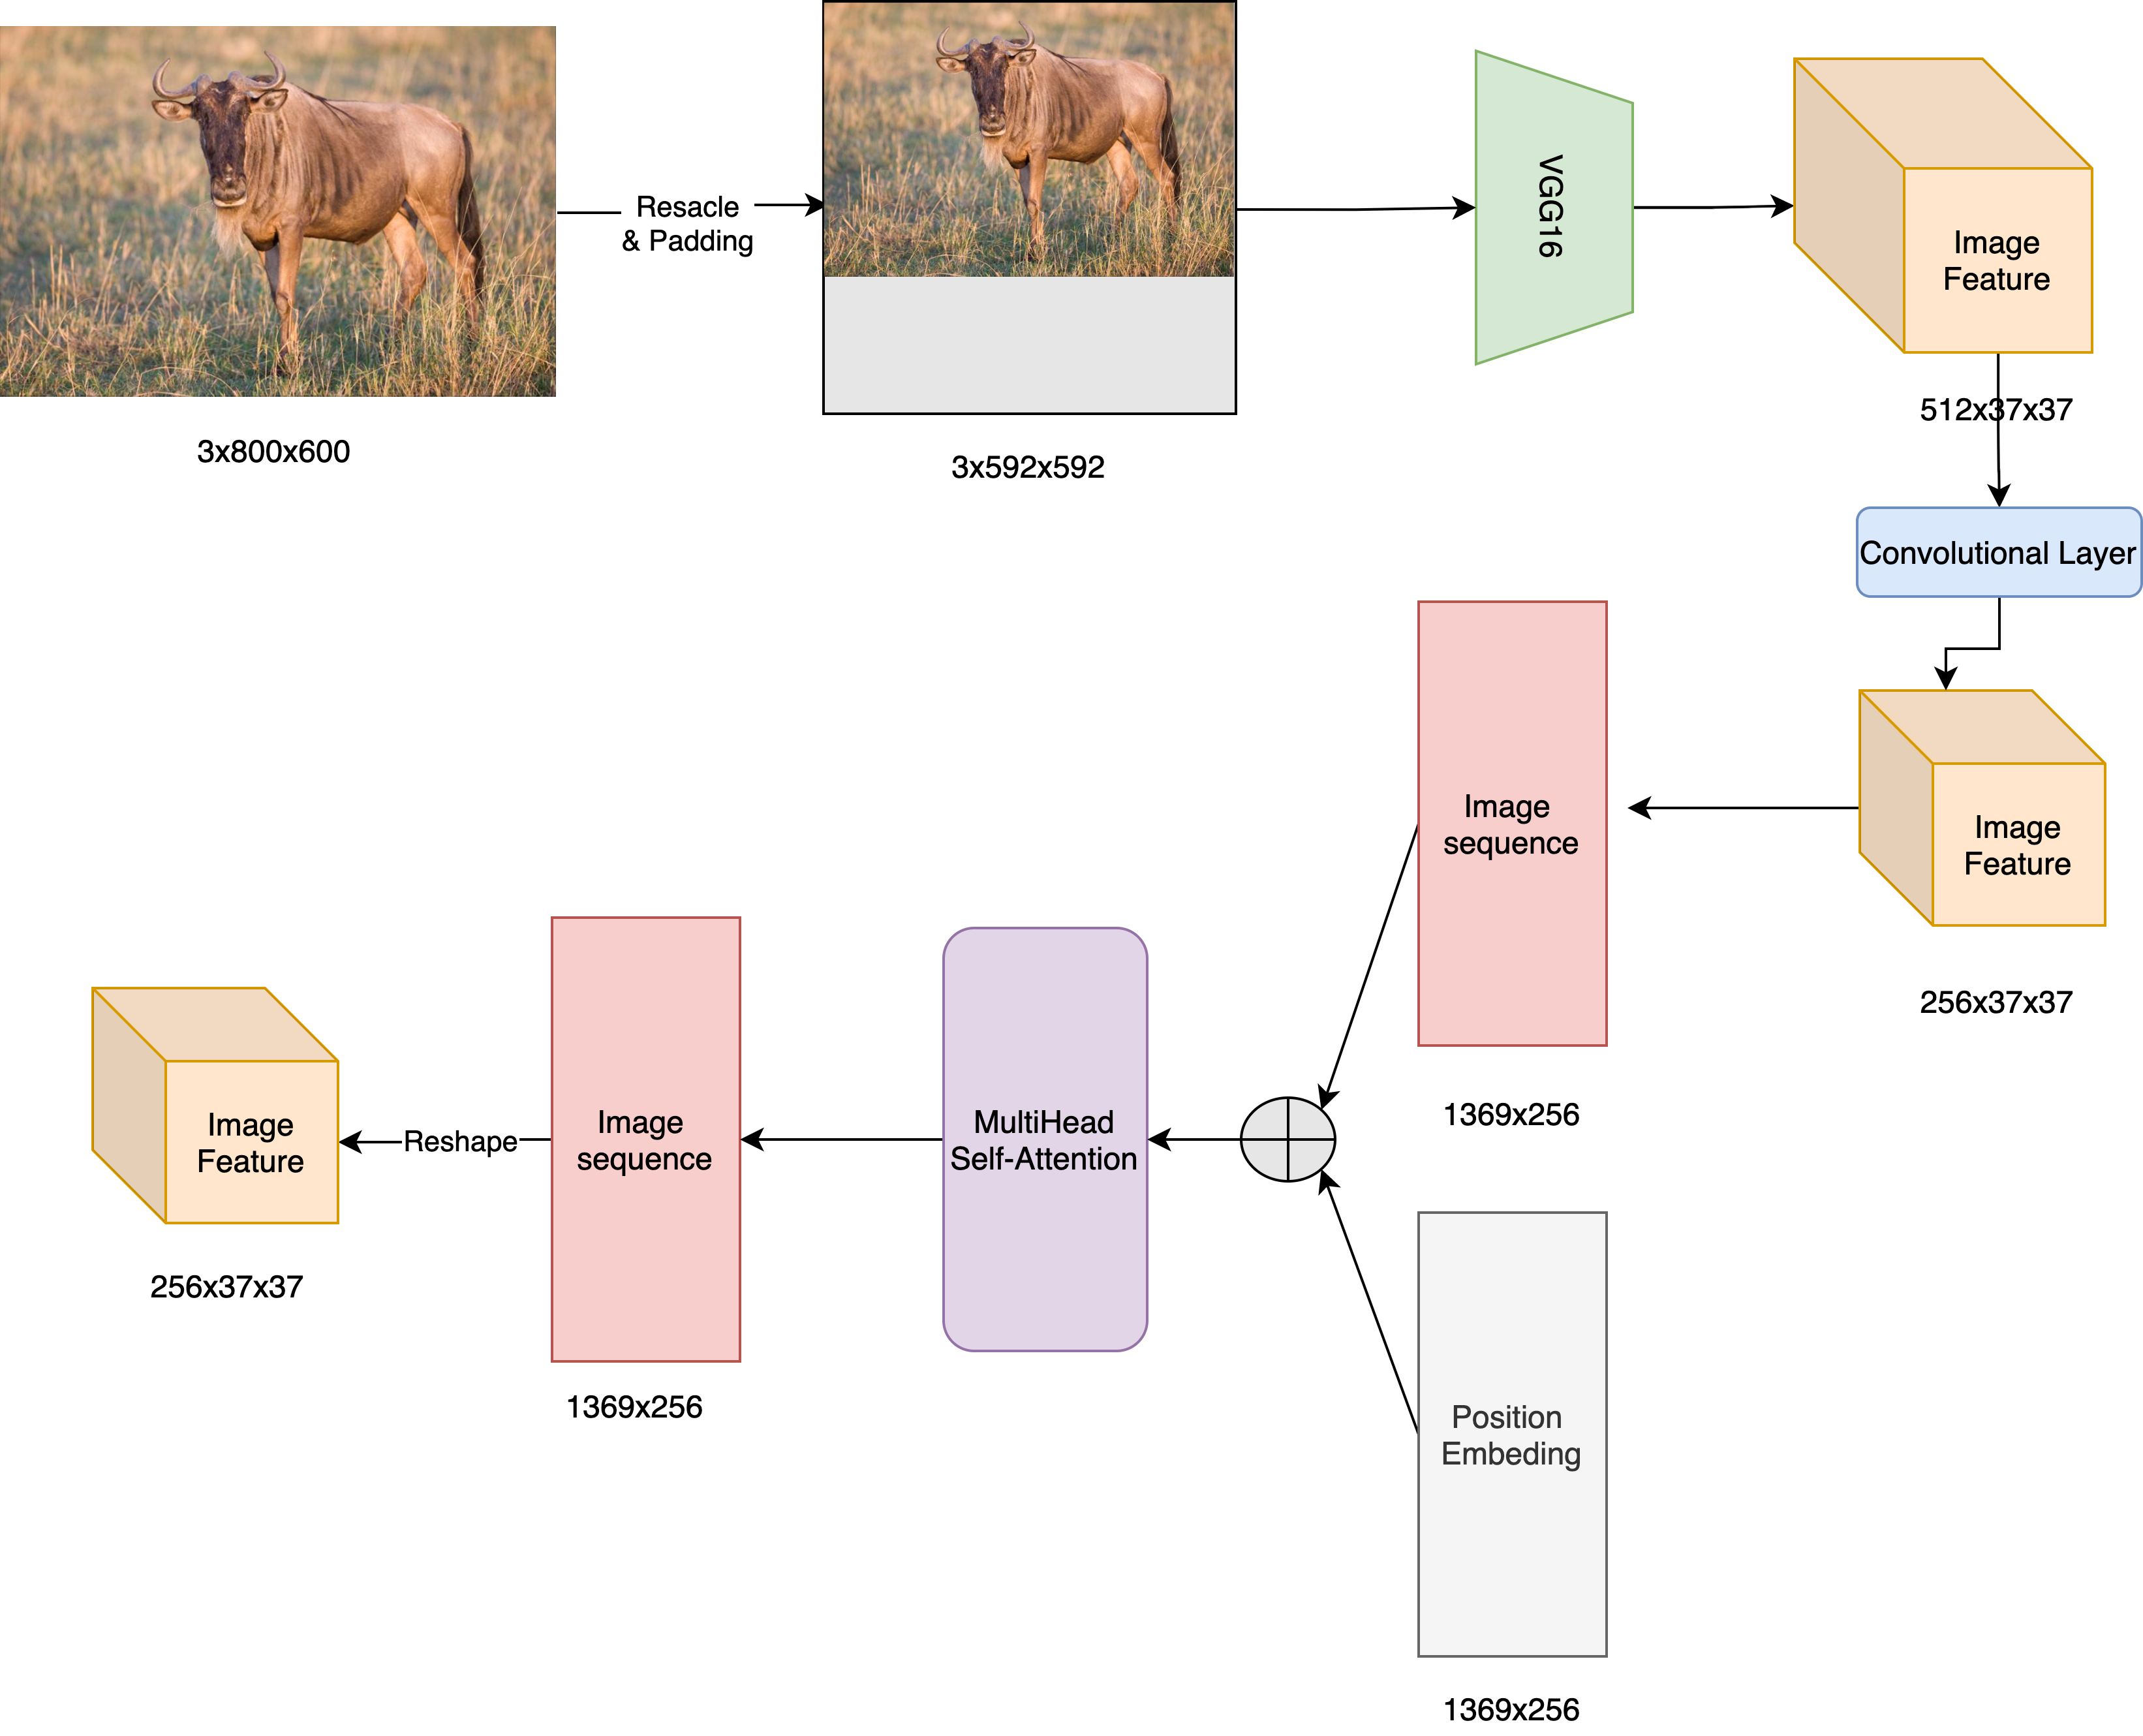
\includegraphics[width=0.9\linewidth]{figures/img_feat_baseline}
	\caption[Generation of Image Feature Map]{Illustration of the generation of image feature maps.}
	\label{fig:imgfeatbaseline}
\end{figure}


%Ours Encoder is a MultiHead Self-Attention module, whose input is an image sequence tensor plus a  Position Embedding tensor. Different from the processing of sequence signals by the RNN network, the Self-Attention module processes the sequence in parallel, so it does not know the order of the sequence, we need to add position information to the original sequence.  we are processing two-dimensional image information, thus we need to add two-dimensional position information for each pixel. We use Equ.~\ref{equ:position_embedding} to encode the position of the picture pixels.

\label{sec:objectdecoder}
\subsection{Object Decoder }

A object decoder contains three multi-head attention modules, which can extract the object features and compute the visual context between objects. The object query should redesigned to adjust different evaluation models in visual relation detection.

\begin{figure}[tbph!]
	\centering
	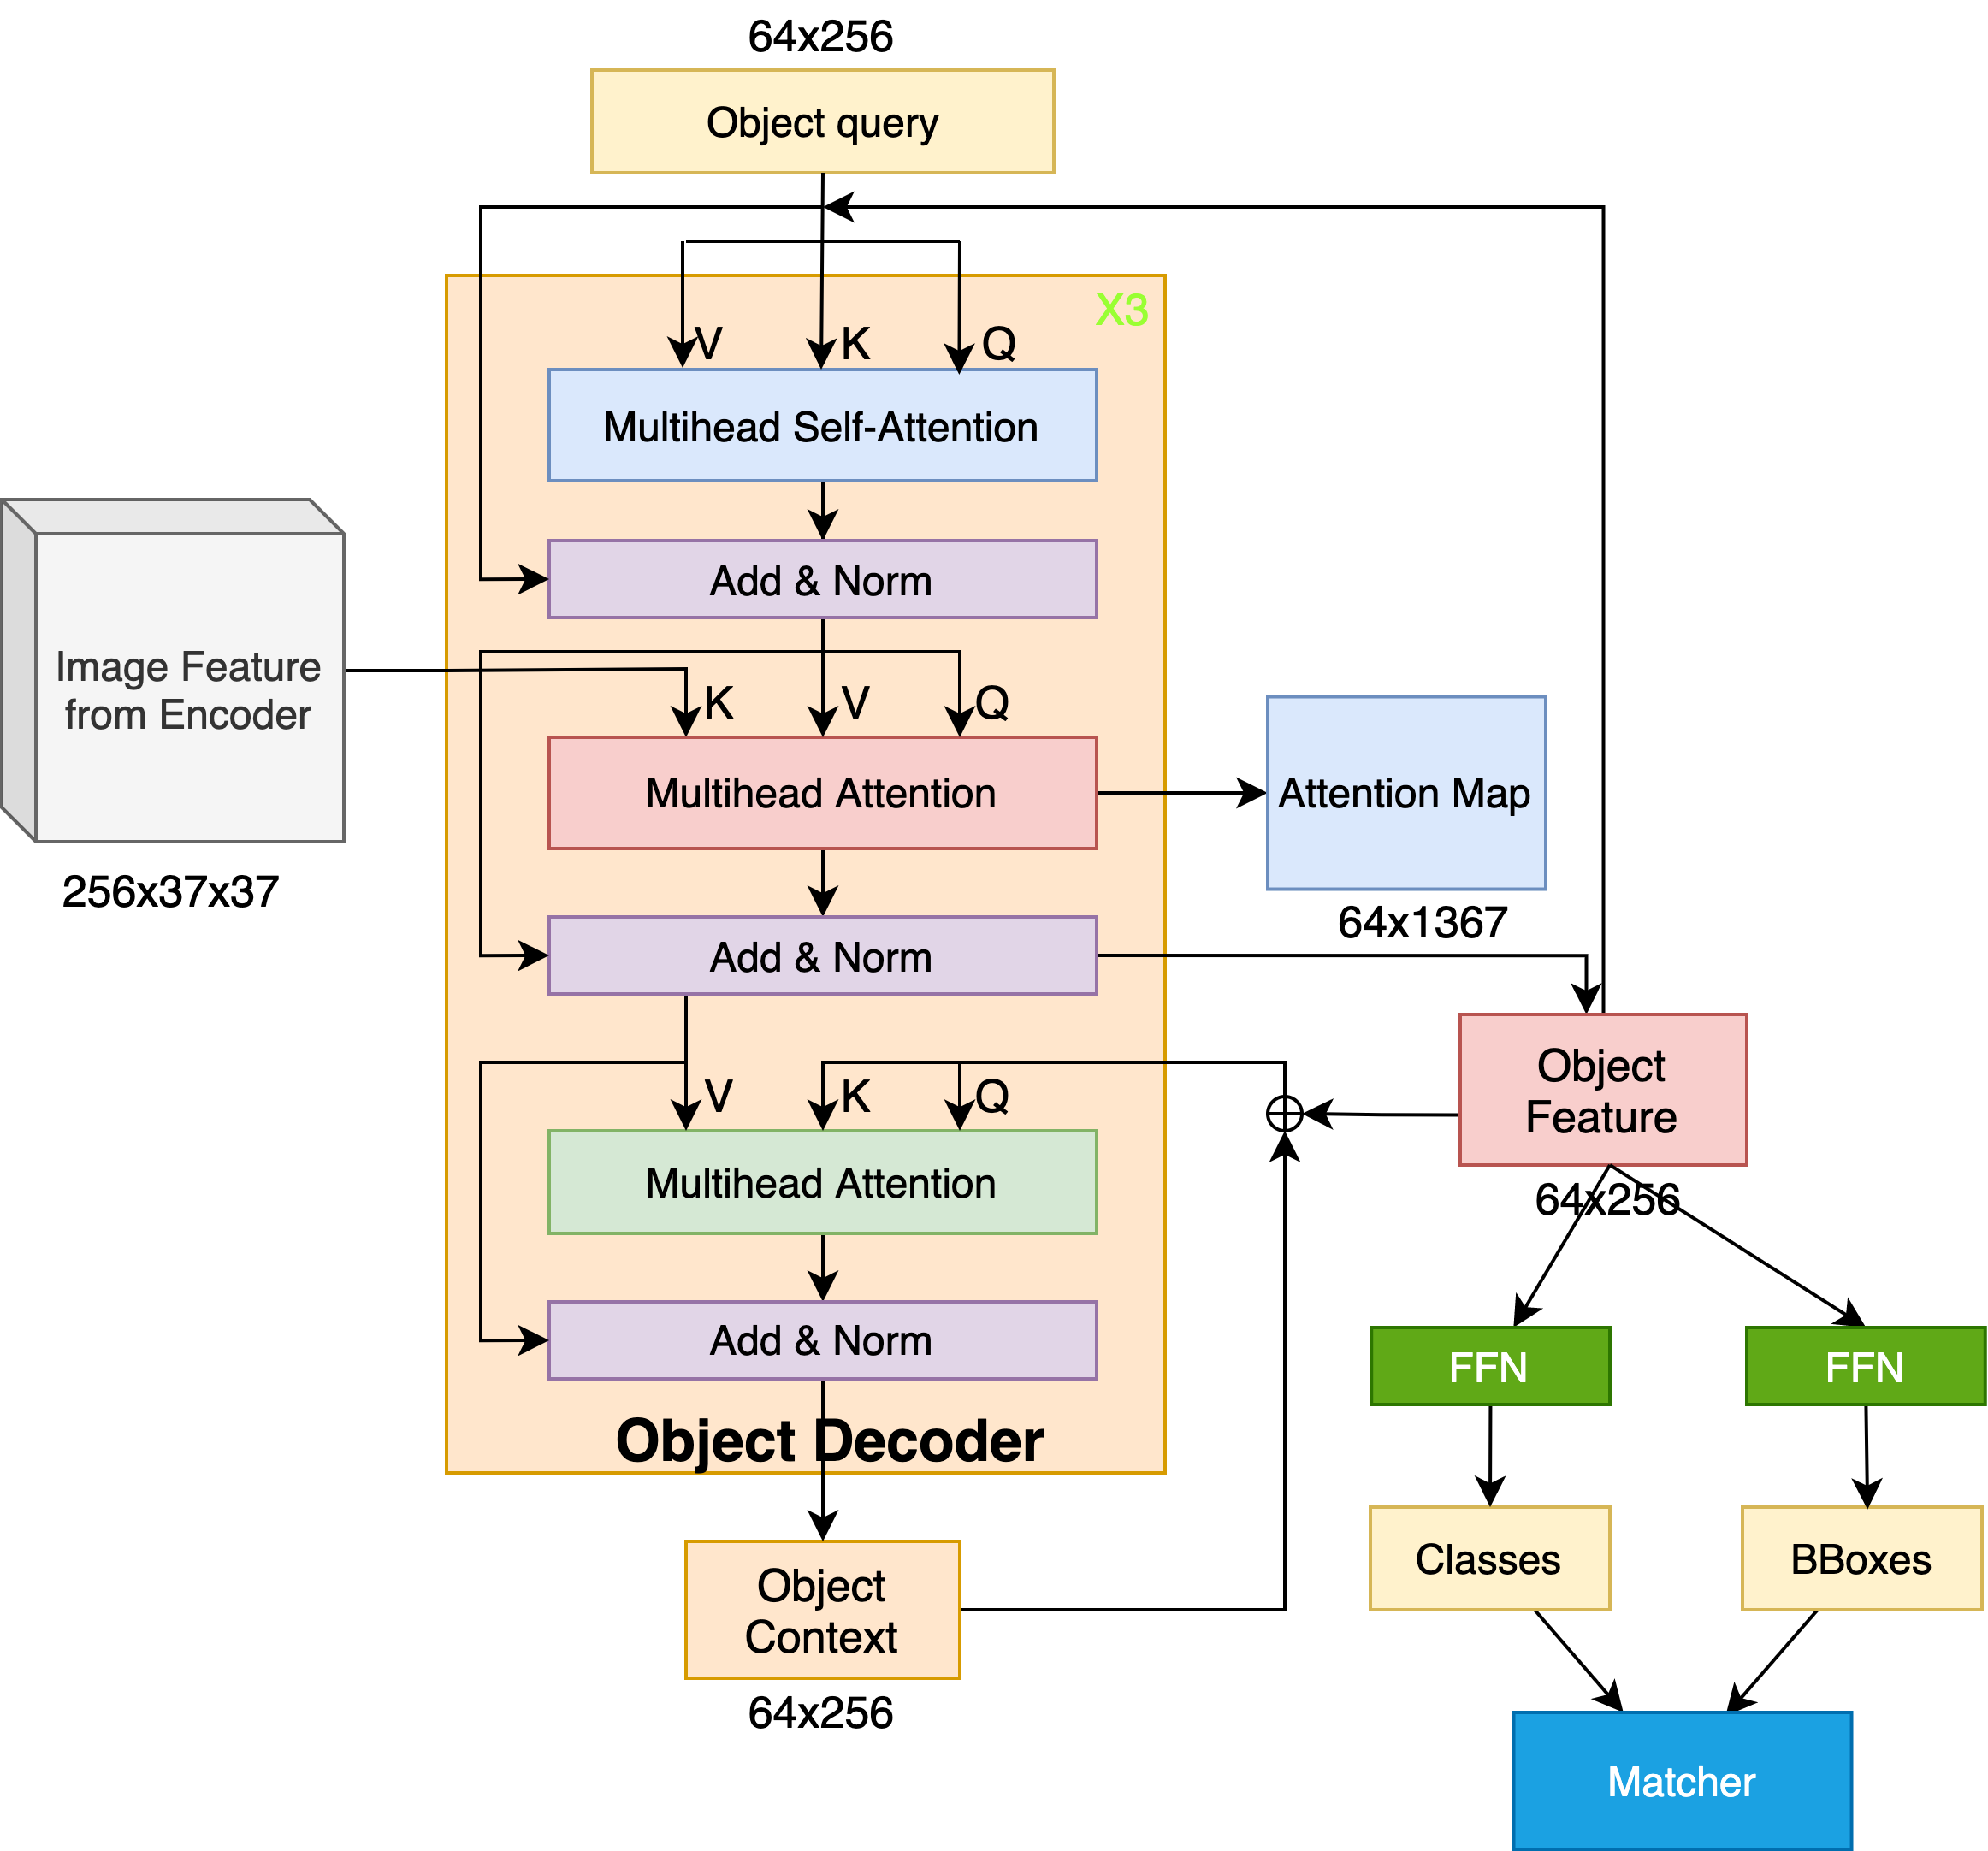
\includegraphics[width=0.9\linewidth]{figures/object_decoder}
	\caption[Illustration of the Object Decoder]{The architecture of the Object Decoder, it consists of three Multihead Attention modules, it has three outputs: Attention Map, Object Feature and Object Context.}
	\label{fig:objectdecoder}
\end{figure}


Figure~\ref{fig:objectdecoder} shows the detailed structure of the object decoder. It is very similar to the original transformer, except that a multi-head attention module is added at the end (the light green part in the figure). For the three evaluation models, this object decoder has different settings, as shown in the Table~\ref{tab:objectdesetting}:
\begin{itemize}
	\item  Predicate classification (PredCLS) is given the bounding boxes and labels of each object, and it extracts the object feature with a box query. Because of the consistency of feature and query, a bipartite matching is unnecessary.
	\item Scene graph classification(SGCLS) is given the bounding boxes and it also extracts the object feature with a box query. But it need to classify the objects with a feed forward network(FNN) to get the object labels. A bipartite matching is not necessary either.
	\item Scene graph detection(SGDET) is given only an image, no other known information, so we use the learnable query in DETR to get the object feature. Then FFN performs class classification and bounding box regression prediction, and finally the best match is found through the Hungarian algorithm in Matcher.
\end{itemize}

\begin{table}[h]
	\centering
	\begin{tabular}{l|ccc}
		\hline
		& PredCLS     & SGCLS       & SGDET           \\ \hline
		object query     & box query & box query & learnable query \\
		class classification & no          & yes         & yes             \\
		boxes prediction & no          & no          & yes             \\
		need matcher     & no          & no          & yes             \\ \hline
	\end{tabular}
	\caption[The setting of the object decoder]{The setting of the object decoder.}
		\label{tab:objectdesetting}
\end{table}




%%\subsubsection{The overview of Object Decoder}
%As shown in Figure~\ref{fig:objectdecoder}, our decoder structure is similar to the decoder structure in the traditional transformer~\cite{vaswani2017attention}. The difference is that we added a new Multihead Attention  (see the light green part in  Figure~\ref{fig:objectdecoder}). module after the second MultiHead Attention module. In addition, we adopted the Multihead Attention of 8 heads 3 layers. We have also made changes to the object query, which we will explain in detail in the following part.



%We obtained the object feature and an attention weight map in the second Multihead Attention module (see the red part in the middle of Figure~\ref{fig:objectdecoder}). Obtain the object context through the third Multihead Attention module. This means the context of one entity to other entities. For example, we have 10 object entities in a picture. The attention map generated by the second Attention module is the effective part of $ 10 \times 10 $. Of course, the size of the attention map should be $  64\times 64 $ showed in Fig.~\ref{fig:objectdecoder}, but we only have 10 valid entities and the other 54 will be filled with 0 .So the attention map will have an effective part of $ 10 \times 10 $. Its meaning is the attention weight of an entity to other entities, including itself, that is, we have obtained a global context.It is worth mentioning that in the first layer of the Object Decoder operation, we initialize the object context to all zero tensor.


%%We can simply derive each output through Equ.~\ref{equ:self_attention}. We set the image feature from encoder be $f_{img}$, the Object Feature is $ f_{obj} $ ,the object context is $ C_{obj} $, and the attention map from the seconde Attention module is$  Att $.



\subsubsection{Object query}
Two object queries mentioned above are box query and learnable query. The learnable query is referenced from DETR and it is the weights of an embedding layer. The interpret ability of this query so poor that it has no actual physical meaning.It is only suitable for the evaluation model of scene graph detection to extract object visual features for object detection. This has been verified in DETR, and the object detection is very successful. But it is not applicable to the models of scene graph detection and predicate classification, because an object detection is not necessary to these two models, they are known bounding boxes. Therefore we should redesign a new object query in combination with the known bounding boxes.

\begin{figure}[tbph!]
	\centering
	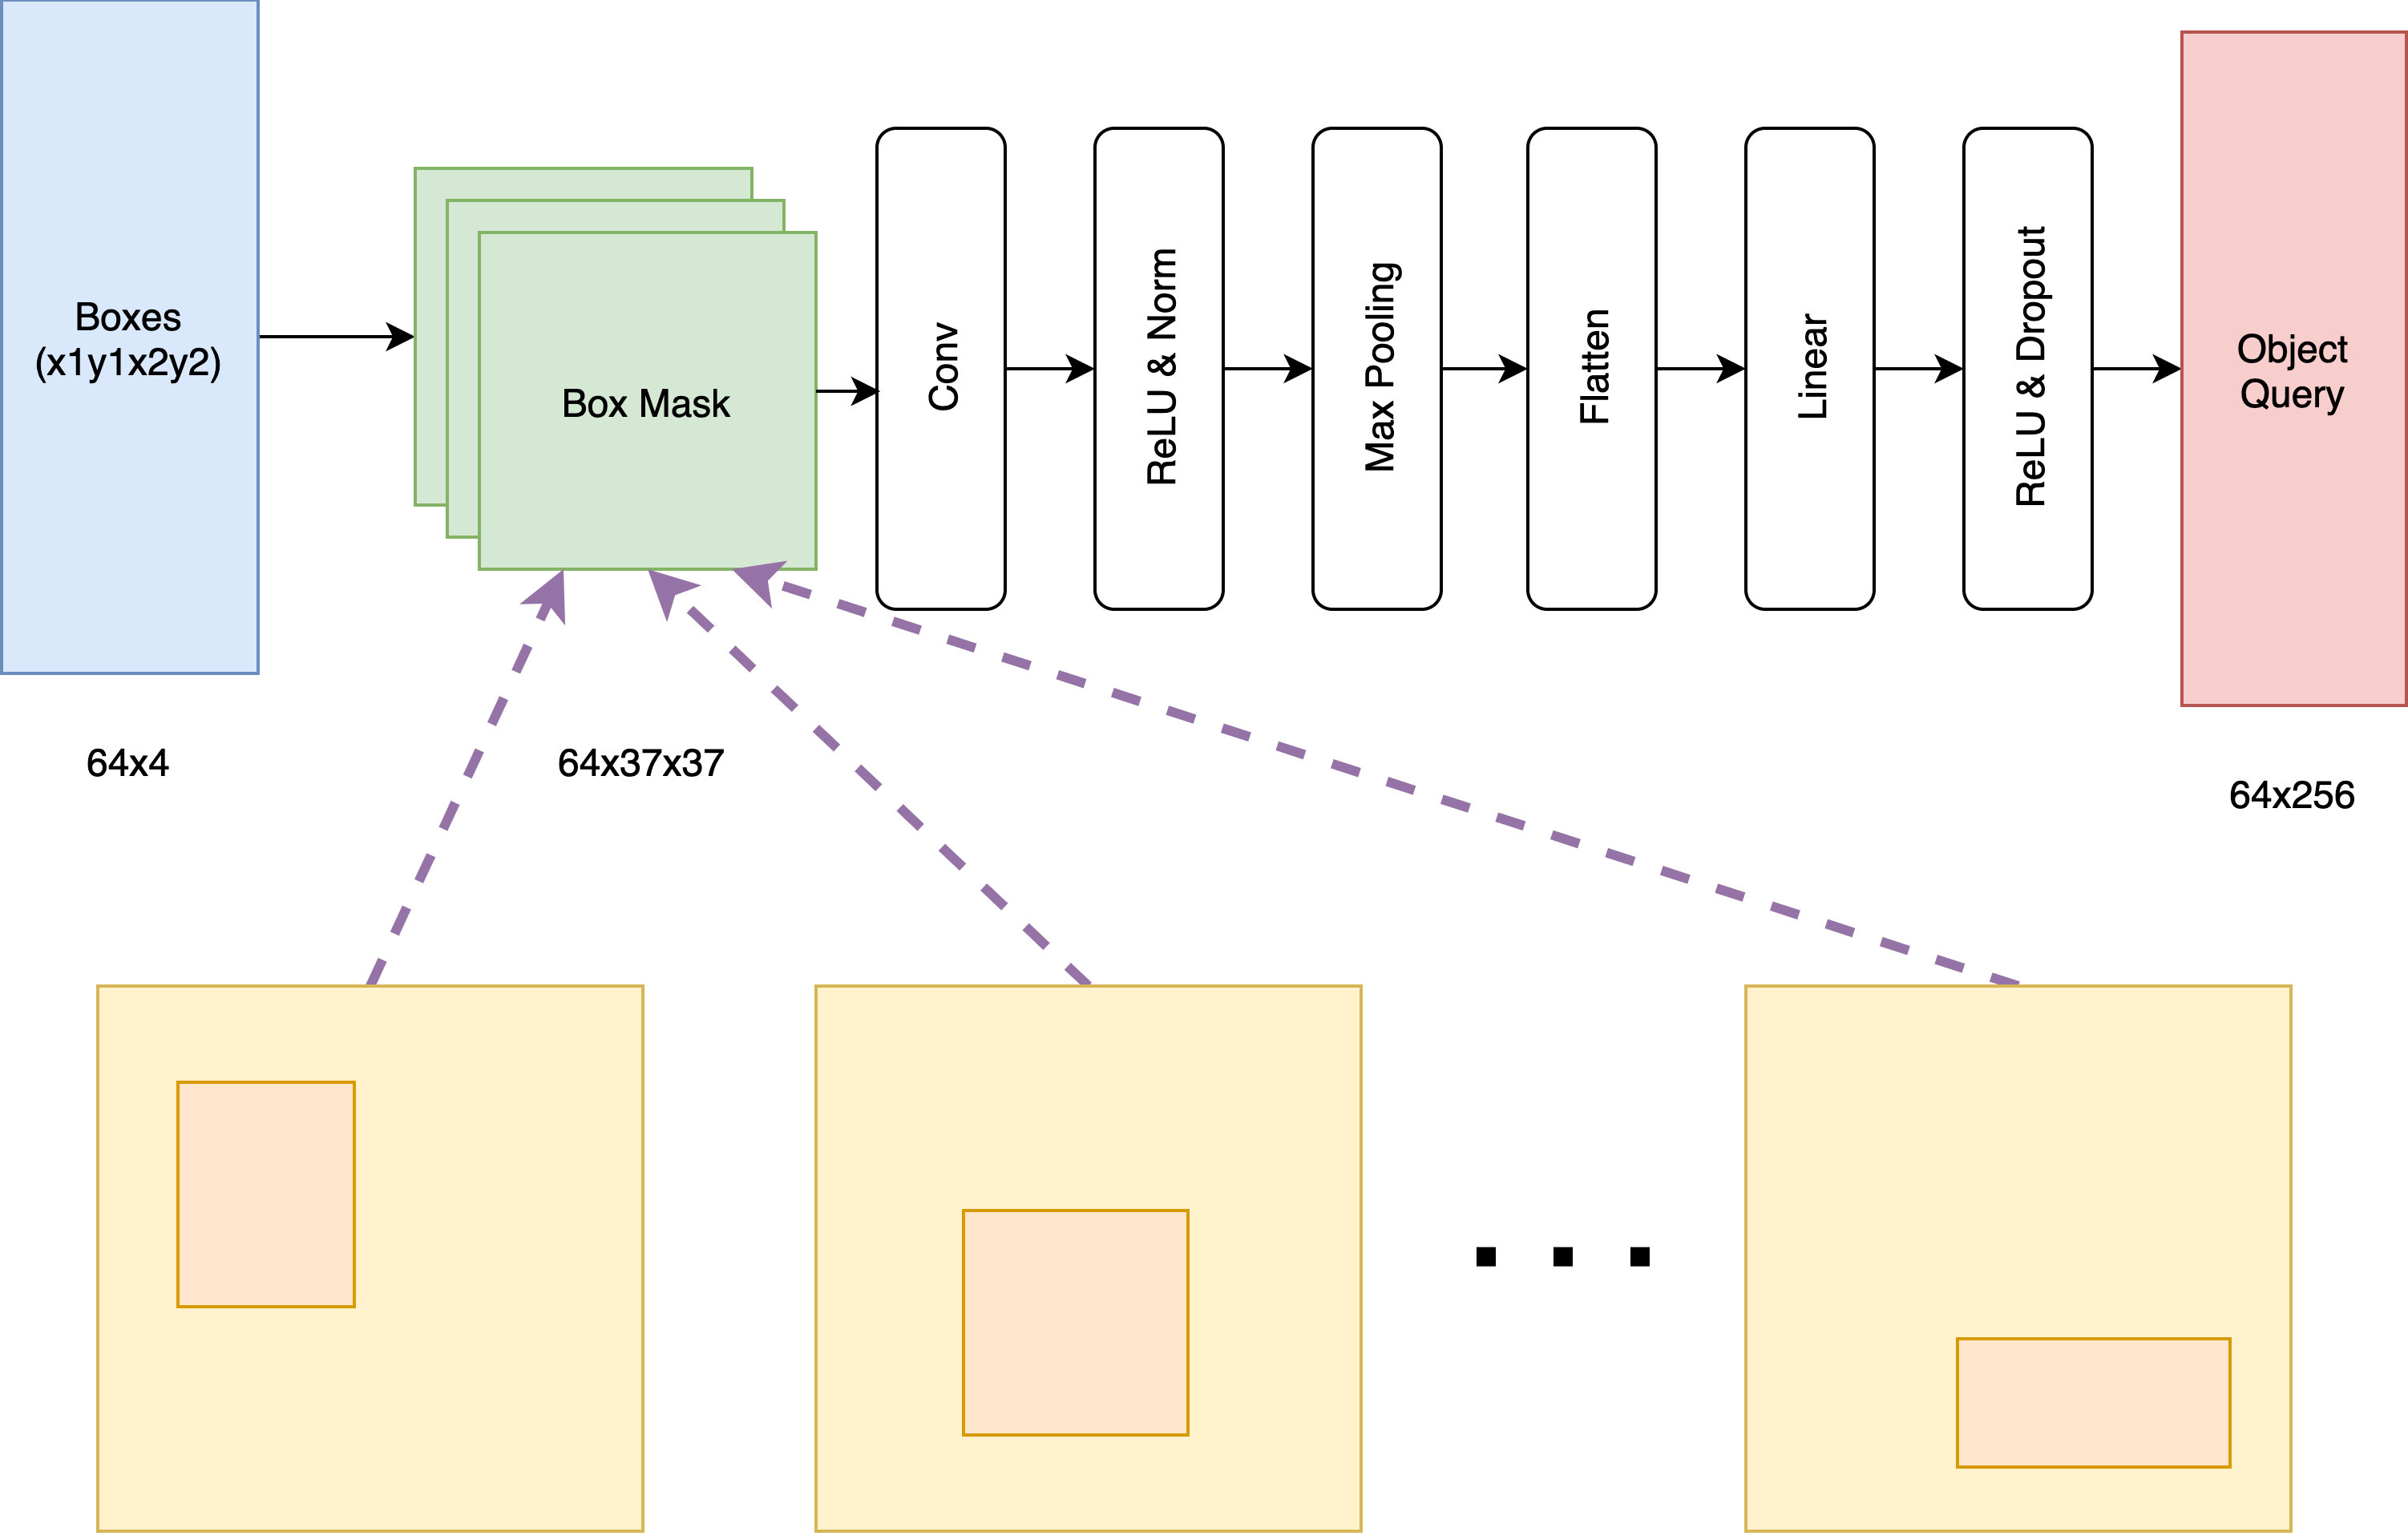
\includegraphics[width=0.8\linewidth]{figures/object_query}
	\caption[Illustration of the object query]{Illustration of the object query.}
	\label{fig:objectquery}
\end{figure}

Figure~\ref{fig:objectquery} is an illustration of a new object query, designed for PredCLS and SGCLS. The bounding boxes are represented as $ (x1y1x2y2) $, which correspond to the upper left corner coordinates $ (x1y1) $ and the lower right corner coordinates $(x2y2)$ of the box respectively.The box mask is defined as a 64x37x37 matrix, the first dimension is set to 64 means that there are 64 prediction slots, because according to statistics in the VG~\cite{krishna2017visual} dataset, a picture has an average of 12 objects, and a maximum of 62 objects, so 64 objects queries are enough to correspond to the objects in the picture. If the number of objects in the picture is less than 64, the extra slots will be filled with zero padding.

\begin{figure}[H]
	\centering
	\includegraphics[width=0.8\linewidth]{figures/box2feature}
	\caption[The process to obtain the box mask]{The process to obtain the box mask.}
	\label{fig:box2feature}
\end{figure}
In Figure~\ref{fig:box2feature}, the initial box mask is an all-zero matrix, and the bounding box $ (x1y1x2y2) $ is projected into the box mask, the coordinates is $ (x1'y1'x2'y2') $, and the value of the corresponding area is set to 1, the orange area of the left picture in Figure~\ref{fig:box2feature}. Then the mask matrix is subtracted by 0.5 to get the result as shown in the right picture of Figure~\ref{fig:box2feature}. which means that the selected orange area, is $ 0.5 $ and the unselected yellow area, is $ -0.5 $. Then the obtained box mask is sent to a convolutional layer to extract features, and then through a series of operations as shown in Figure~\ref{fig:objectquery}, the final object query with a size of 64x256 is obtained.

The box query designed in the above way has more physical meaning, it corresponds to the spatial position information of the object, and the object feature corresponds to each object one by one, so the bipartite matching operation is omitted.  Because the object query is obtained through bounding boxes, this box query is not applicable to scene graph detection that does not provide bounding boxes.

%In related papers (such as DETR~\cite{carion2020end} and Deformable DETR~\cite{zhu2021deformable}), using transformers for object detection, in addition to only one picture information, it is necessary to make predictions of classes and bounding boxes, so they use the learnable obeject query: they used the weight of an embedding layer as the object query. First of all, the interpretability of this query is very poor and has no actual physical meaning. Moreover, in the three tasks of VRD: SGCLS provides the entity's bounding box information, and even the PREDCLS task provides category information. Therefore, in these two tasks, we can make full use of the known information and propose a new entity encoding method to use as an object query.Since the known conditions provided by the three tasks of VRD are not the same, we use different queries.
%
%
%In this thesis, we propose a custom object query for PREDCLS and SGCLS tasks, as shown in Fig.~\ref{fig:objectquery}. In these two tasks, the bounding box is known information, so we first project the box information of the form $ (x1y1x2y2)  $(where$ [x1,y1] $ is the coordinate of the upper left corner of the box, and $ [x2,y2] $ is the coordinate of the lower right corner of the box)on a size of $ 37 \times 37 $ mask. We set the selected area(the orange area in the figure) be $ 0.5  $ and the unselected area (the yellow area in the figure) be $ -0.5 $. After extracting spatial information through a convolutional layer, the max pooling layer scales the tensor size, and finally transforms it to the size we need $ 64 \times 256 $ through a linear layer.
%
%For the task SGDET, we do not have the information of the bounding box, so we continue to use the learnable object query, that is, use the weight of an embedding layer with a size of $ 64 \times 256 $.
%
%For the size of the object query, we chose $ 64 \times 256 $, because according to our statistics on our dataset, each image has a maximum of 62 bounding boxes, and it has an average of 11.87. So we choose 64 queries will be greater than the maximum number of the entity. 
%





\subsubsection{Generation of Object Feature Maps }

As shown in Figure~\ref{fig:objectdecoder}, object query and image feature are input to object decoder, and output is object feature and object context. The object feature is obtained by performing multi head attention on object query and image feature. Among them, query \textit{Q} and value \textit{V} of the attention module are object query, and key \textit{K} is image feature.Each query will be calculated with the feature of the entire image to find the most concerned part in the image for the object, which can be reflected in the attention map. Different from the attention map in Sec.~\ref{sec:pixelbaseatt} pixel-wise, this attention is box to pixel. It pays more attention to the pixel representation of this object in the image. 

Since the attention map will reflect the most concerned pixels of this object in the image, it can be seen from Equ.~\ref{equ:self_attention} that the weights of the object feature is the values in the attention map. Different from the object features extracted by ROI Align, the features extracted by the multi-head attention module are considered globally. ROI Align only pays attention to the area of the object, and does not consider the area outside the object, while multi-head attention focuses on the area of the object, and pay little attention to the area outside the object.

When SGDET detects objects, it uses  the learnable query to look up the object feature, and obtains the distributions of classes and bounding boxes through two FFNs. Finally, through the Hungarian matching algorithm the optimal matching can be found with the smallest cost. The process is the same as DETR, see Sec.~\ref{sec:matchingloss} for details.
%As shown in Figure~\ref{fig:objectquery}, we obtain the object feature through the first two Multihead Attention modules, and the process is similar to that in DETR. The difference is that we use different object queries for different tasks, as mentioned above.
%
%For tasks PREDCLS and SGCLS, we use custom object querries. Since the query and bounding box information correspond one-to-one, the generated object features are also one-to-one correspondence, which we will prove through experiments in the next chapter.
%
%For the task SGDET, we use a learnable query to generate the object feature, which has no corresponding relationship, and we use the Hungarian matching algorithm to find the optimal object feature with the smallest cost.


\begin{figure}[h]
	\centering
	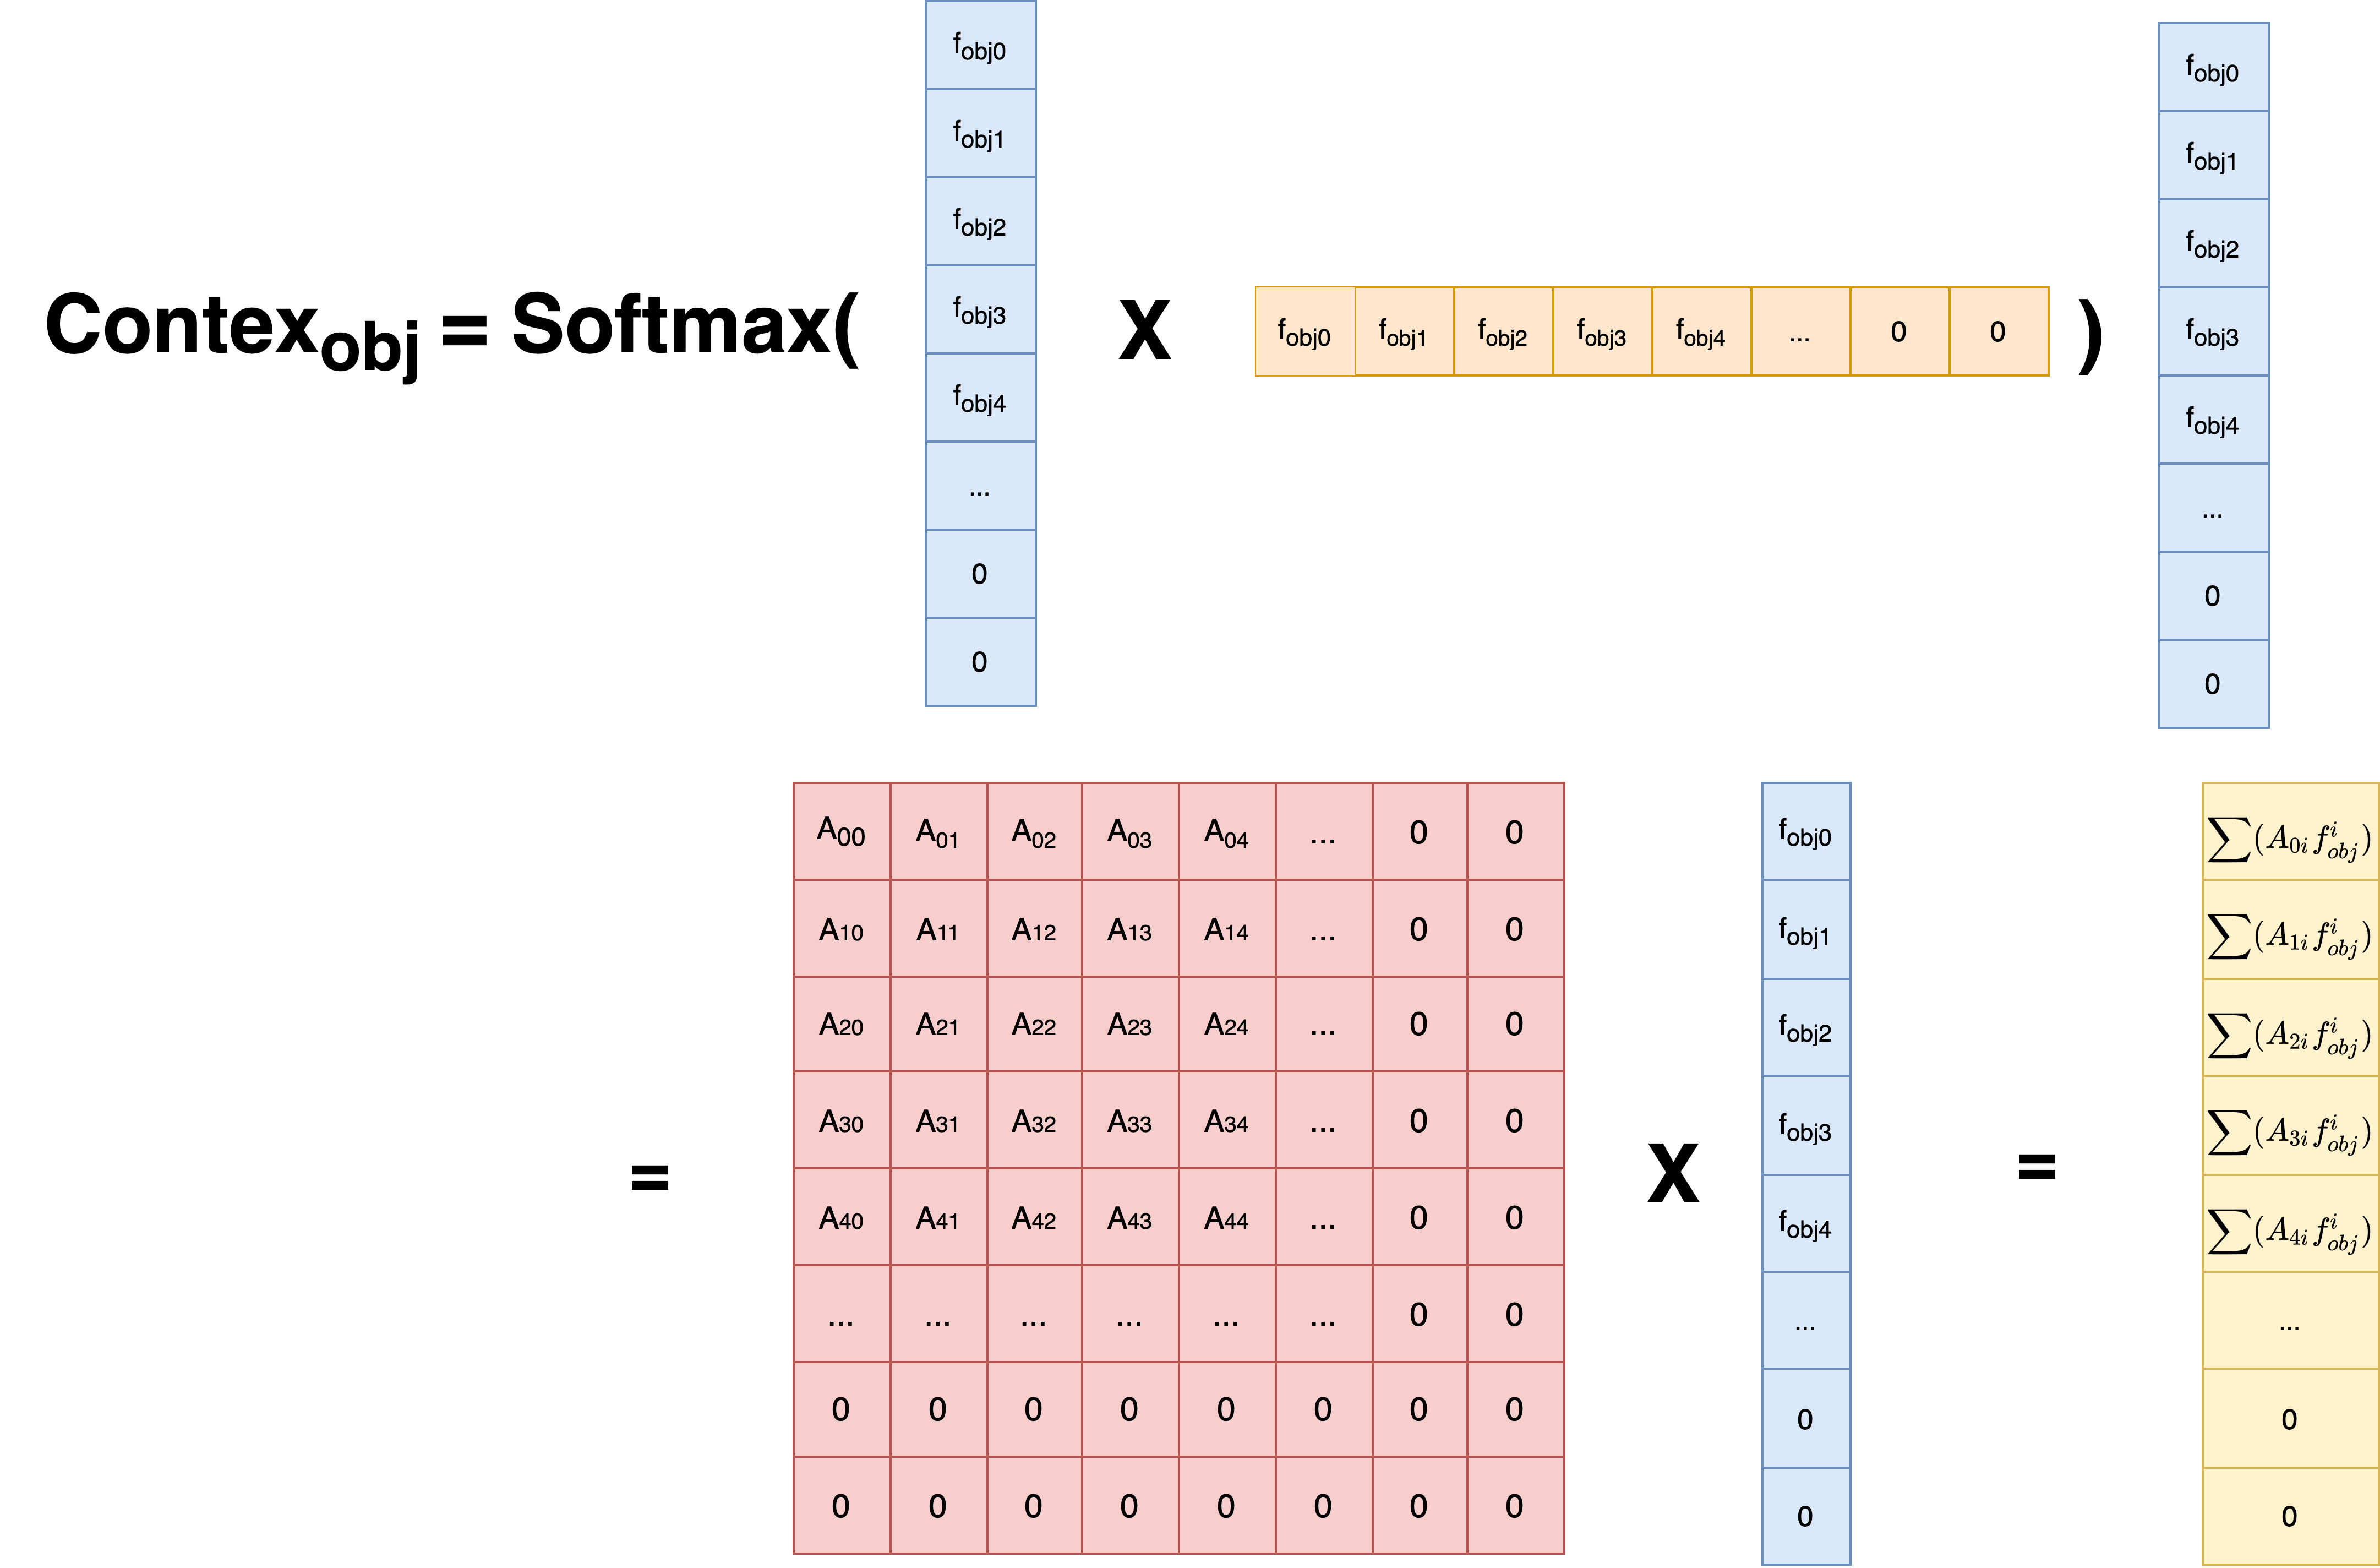
\includegraphics[width=1\linewidth]{figures/obj_context}
	\caption[A simple example of the  Object Context generation.]{A simple example of object context generation. The Object Feature size is 64x256, we assume that this picture has 5 entities, and the remaining 59 objects will be padded by 0.}
	\label{fig:objcontext}
\end{figure}

\subsubsection{Object Context}

As shown in the figure~\ref{fig:objectdecoder}, the object context is obtained in the third multi-head attention module. The specific operation is shown in figure ~\ref{fig:objcontext}. A simple example according to Equ.~\ref{equ:self_attention} is given: Before computing the object decoder for the first time, the object context is initialized to an all-zeros matrix. The blue vector in the figure is \textit{object features}, and its size is 64x256. Assuming that there are 5 entities in the picture, the remaining 59 positions of the feature should be padded by 0. The orange vector is the transpose of \textit{object features}, which is multiplied by the \textit{object features} and then manipulated by the softmax operation to obtain the red matrix \textit{attention map} in the figure with a size of 64x64, which represents the attention between objects, such as $A_{23}$ is the attention from $object_2$ to $object_3$.If $ object_1 $ has a relationship with $ object_2 $ and $ object_3 $, the attention values of  $A_{12}$  and  $A_{13}$  can be higher. In the context of $ object_1 $, the weights of $ f_{obj2}$ and $ f_{obj3} $  should be higher, and the features of other objects should be lower. This characteristic helps the model to predict the relationship better.
Finally, the \textit{attention map} is multiplied by the \textit{object features} to get the yellow vector \textit{object context} in the figure. The context of $object_1$ is $\sum(A_{1i}f_{obj}^i)$, which is the sum of attention between $object_1$ and other $object_i$.

%After softmax, an attention weight matrix of $64\times 64$ (the red matrix in the figure) is obtained, which means the attention between each object pairs. . For example, $A_{23}$ is the attention of $object_2$ to $object_3$, and finally multiplied by the object feature, the object context is computed (the yellow vector in the figure). The context of $ object_1  $is $ \sum_1^{64}(A_{1i}f_{obj}^i) $, that is, the context of $ object_1 $ to other $ object_i $.
%
%When using multi head attention, an attention map is generated, which is the attention of object to object, and it represents the interaction between objects, and also considers the attention of an object to all objects.


%As shown in Figure~\ref{fig:objectdecoder}, we obtain the object context in the third Multihead Attention module. Its specific operation is shown in Figure~\ref{fig:objcontext}. We have given a simple example according to Equ.~\ref{equ:self_attention}. Before computing the object decoder for the first time, we initialize the object context to a tensor with 0. Assuming that we have 5 entities in the picture, before we calculate the context, the object feature size obtained from the previous calculation is $ [64, 256] $, and 59 positions will be paded by $\emptyset$. After softmax, we will Obtain a $ 64 \times 64  $ attention weight matrix (the red matrix in the figure), its meaning is the attention of each object and other objects, such as $ A_{23}$ is the attention of $ object_2 $ to $ object_3 $, and finally multiplied by the object feature we will get the object context (the yellow vector in the figure). The context of $ object_1  $is $ \sum_1^{64}(A_{1i}f_{obj}^i) $, that is, the context of $ object_1 $ to other $ object_i $.




\subsection{Relation Decoder}
The relation decoder in the model is a typical decoder structure, composed of two multi-head attention modules (see figure ~\ref{fig:relationdecoder}), and the relation query is generated by the bounding boxes of the relation pair$<subject,objtect>$.If there are 10 entities, they can have 90 relation pairs, and then 90 relation queries are generated. Select the bounding boxes of each relation pair to generate two boxes mask, and then generate the relation query through a process similar to object query generation (see Figure ~\ref{fig:relationquery}). The only difference is that the input of the convolutional layer becomes two box masks.%卷积层的输入由变成了两个box masks。

The relation context is the context of one relation query to all objects. Object feature $f_{obj} $ can be represented with visual features, spatial features and semantic features: $$f_{obj} = concat(f_{vis},f_{spt},f_{sem})$$ 
The visual feature $f_{ vis}$ is the object feature obtained by the object decoder, the semantic feature $f_{sem}$ is obtained by encoding the category through GloVe~\cite{pennington2014glove}, and the spatial feature $f_{spt} $ Is a feature that contains the spatial location information of the entity, which can be obtained by encoding the bounding box. In this thesis, the attention map obtained in the object encoder also has spatial location information, so the attention map is used to extract spatial features through convolution.


%Our relation decoder is a typical Decoder structure consisting of two Multihead Attention modules(see in Fig.~\ref{fig:relationdecoder}). Our relationship query is customized and generated by the relationship pair $<subject,objtect>$. For example, if we have 10 entities, then we have 90 pairs, and then 90 relation queries are generated. We select the subject bounding box and object bounding box in each pair to generate two box masks, and then obtain the relation query  through the convolutional layer and the linear layer (see in Fig.~\ref{fig:relationquery}).



\begin{figure}[tbph!]
	\centering
	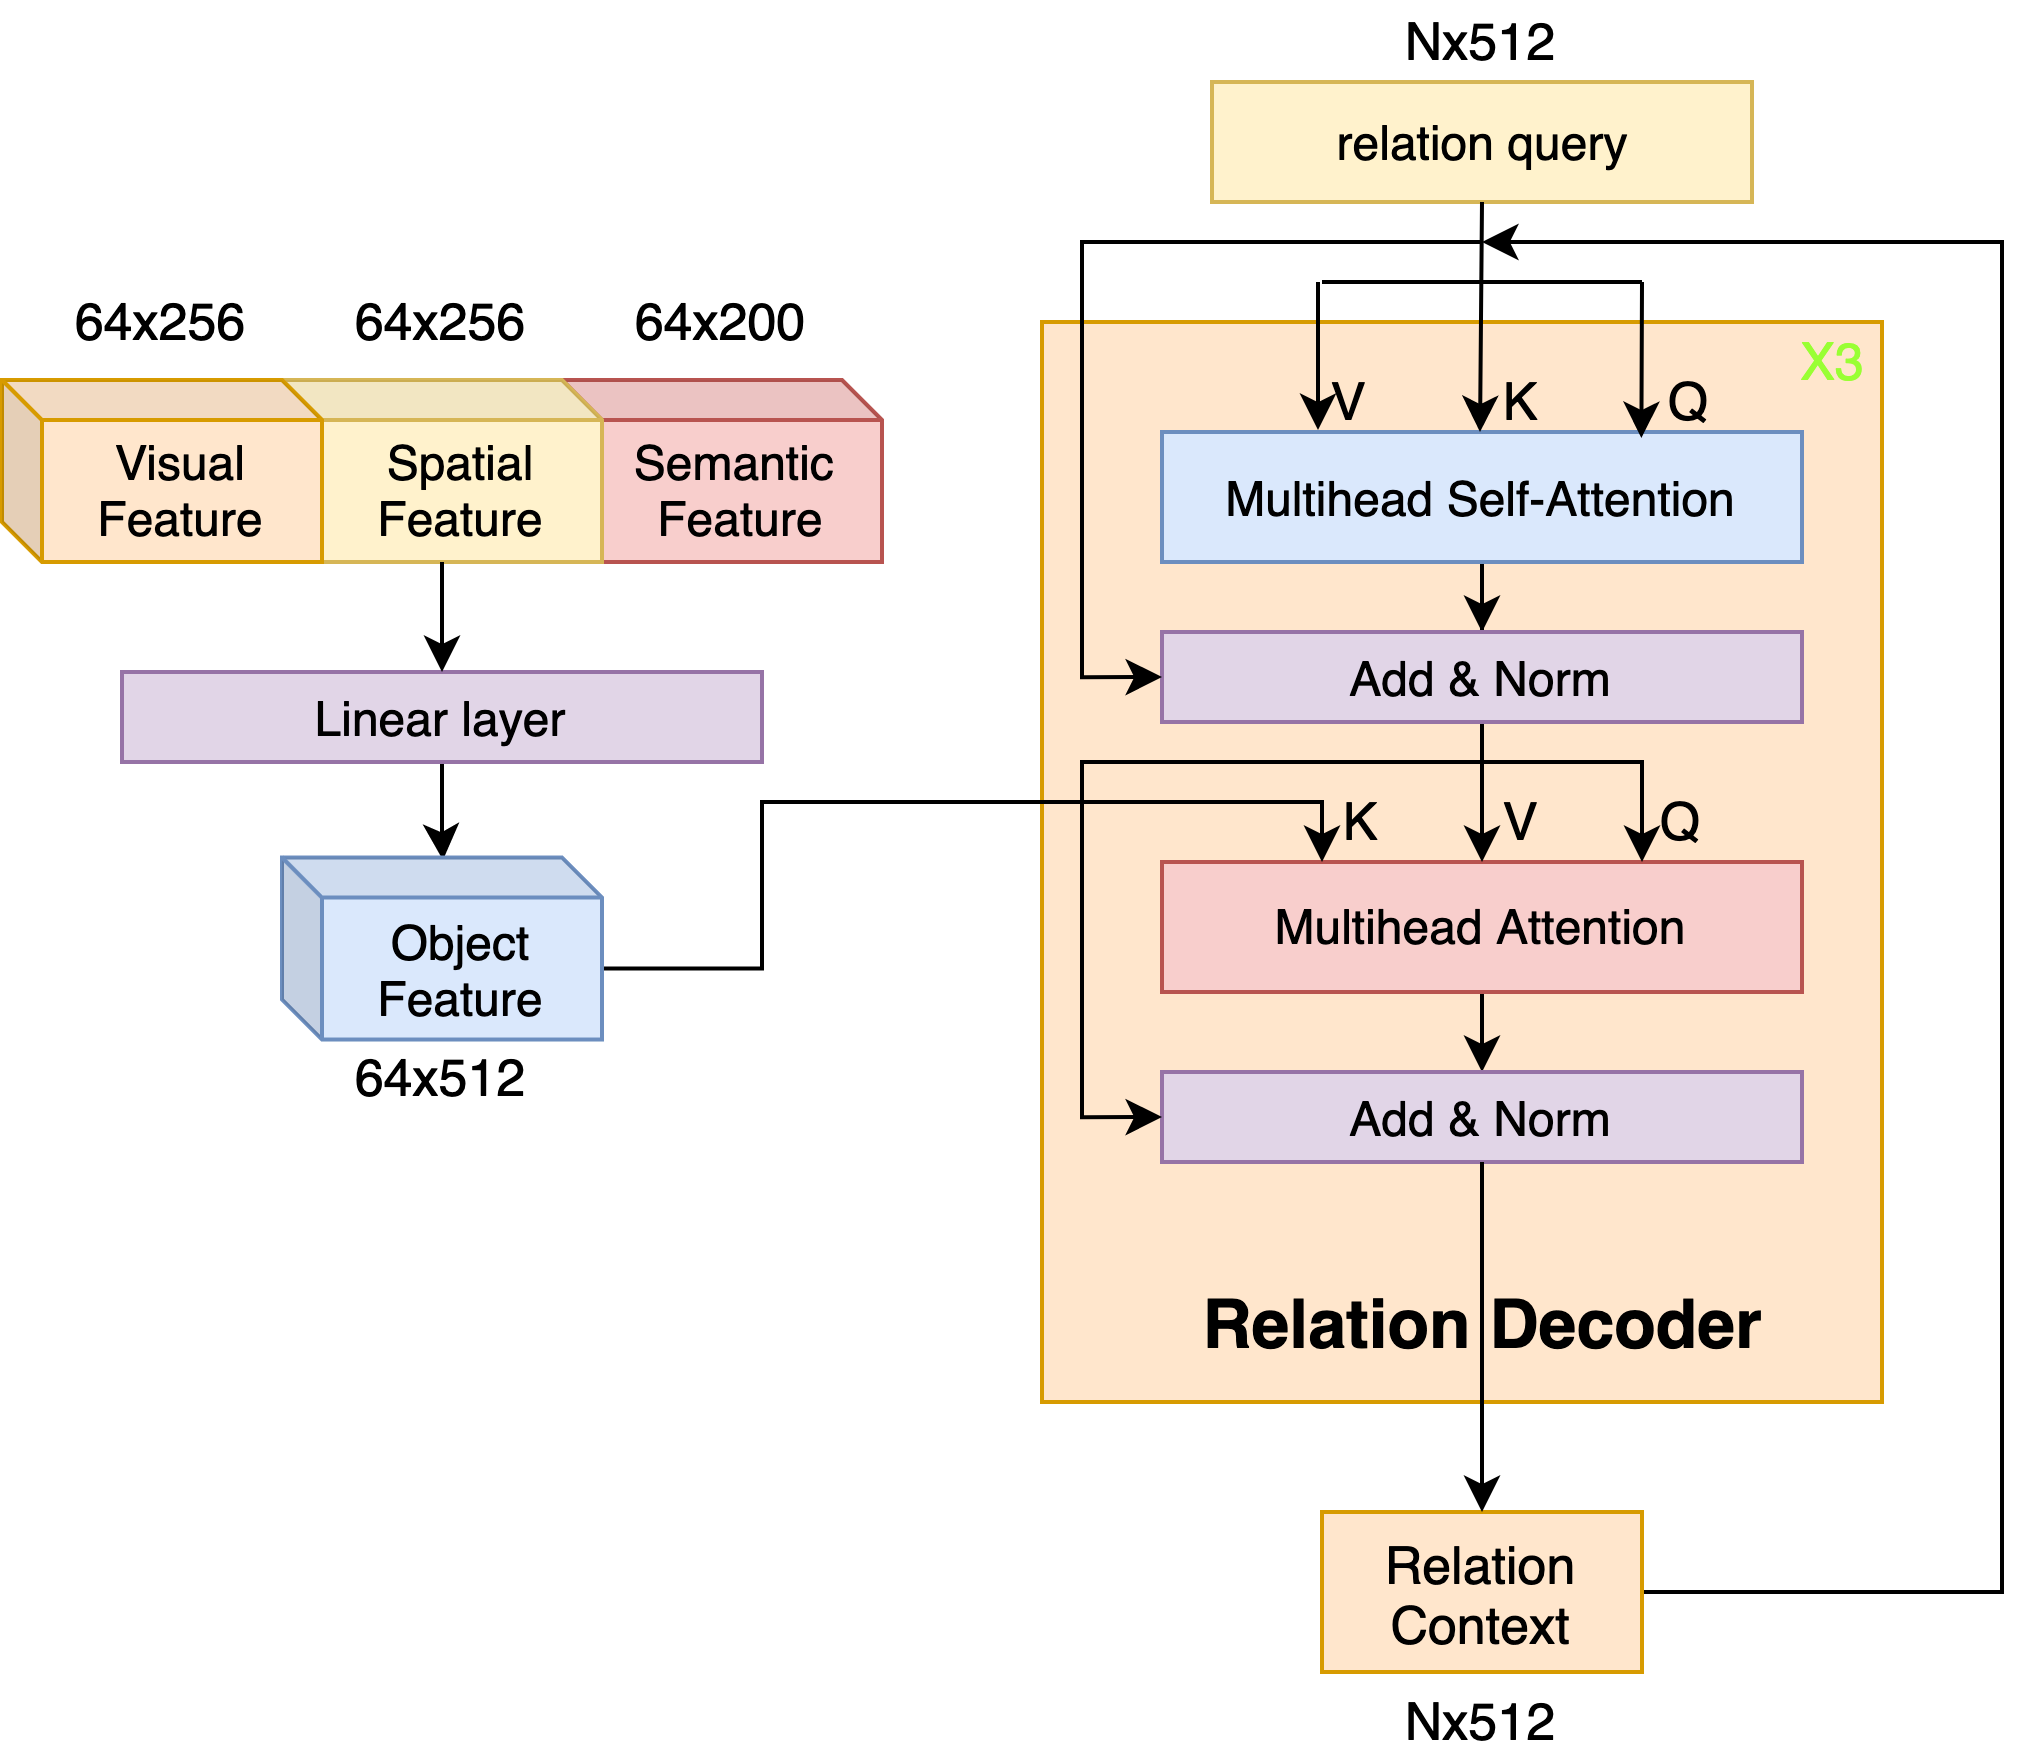
\includegraphics[width=0.8\linewidth]{figures/relation_decoder}
	\caption[Illustration of Relation Decoder]{Illustration of Relation Decoder.}
	\label{fig:relationdecoder}
\end{figure}

\begin{figure}[tbph!]
	\centering
	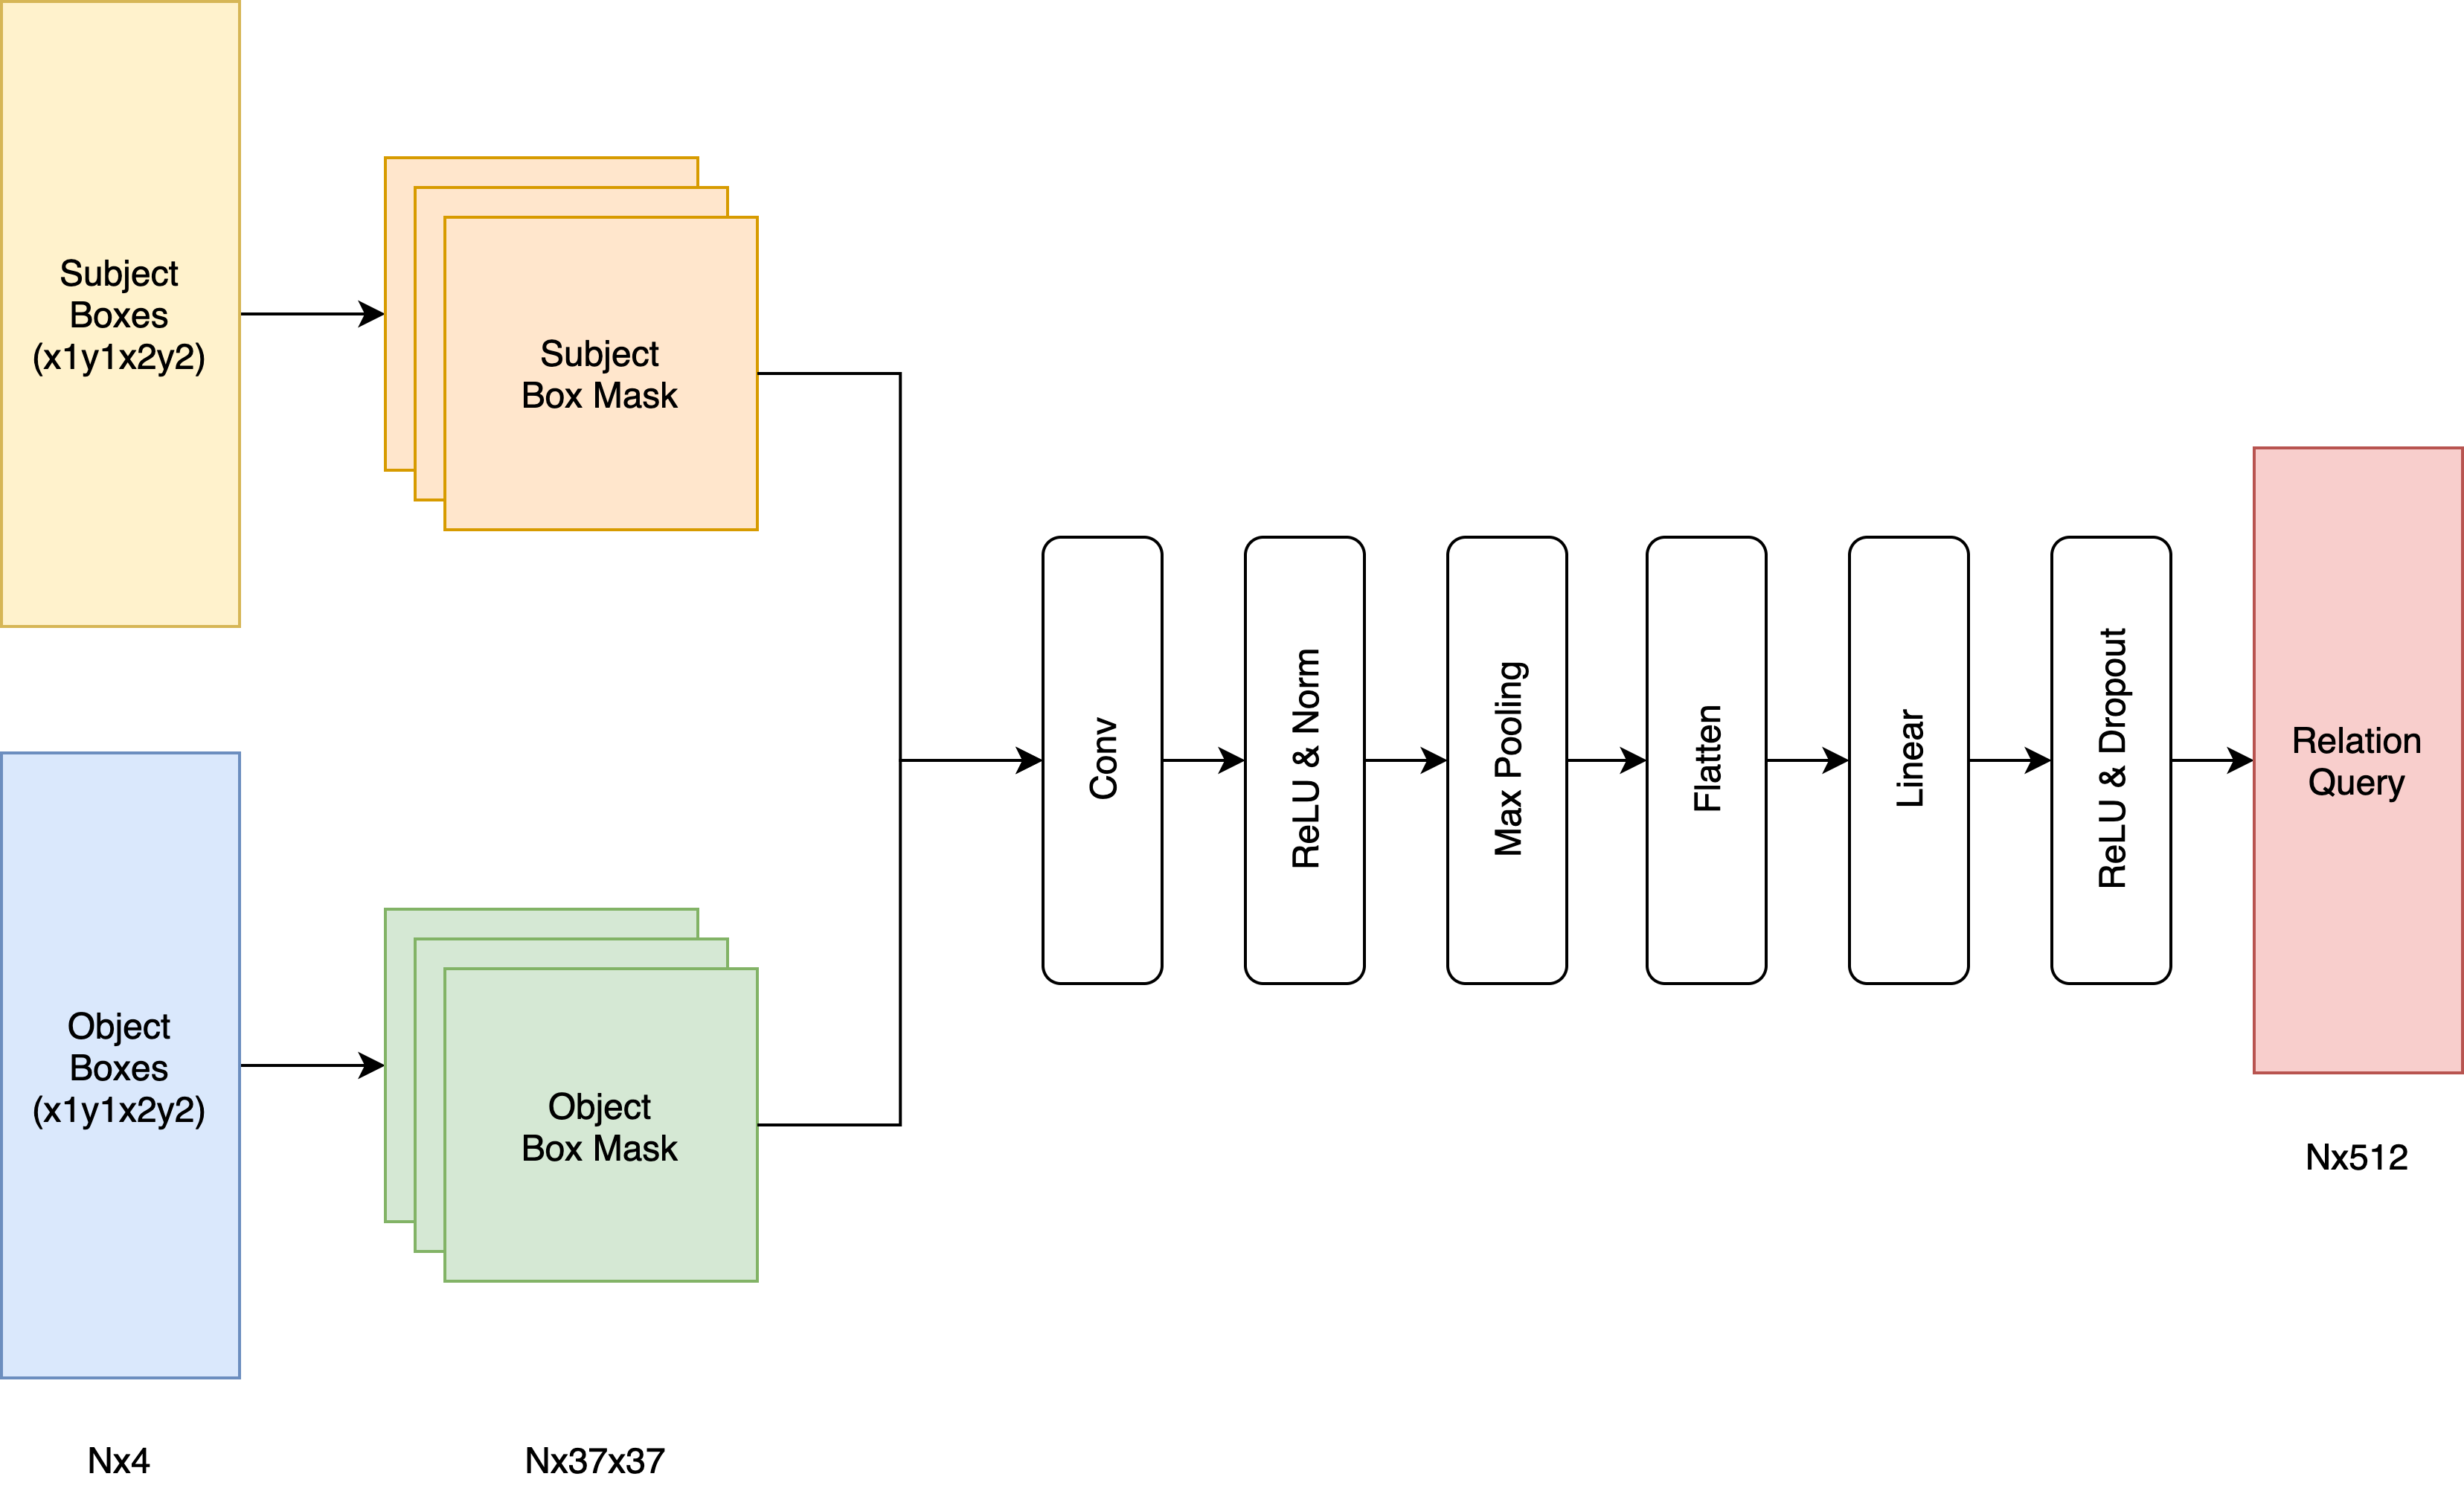
\includegraphics[width=0.8\linewidth]{figures/relation_query}
	\caption[Illustration of the relation query]{Illustration of the relation query. N is the number of the relation pair.}
	\label{fig:relationquery}
\end{figure}

%Our relation context is the context of each relation for all objects. We use visual feat, spatial feature and  semantic feature to jointly represent object: $$f_{obj} = concat(f_{vis},f_{spt},f_{sem})$$ Among them, the visual feature $f_{vis}$ is the object feature obtained through the object decoder. The semantic feature $ f_{sem} $ is a tensor containing the semantic information of entities obtained by encoding the category through GloVe~\cite{pennington2014glove}. The spatial feature $ f_{spt} $ is a feature that contains the spatial location information of the entity. We can get it through the bounding box. In our thesis, the attention map obtained in the object decoder also has good spatial location information, so we also use the extraction of the attention map to obtain the spatial feature.



\subsection{Predicate Classifier}

 \begin{figure}[h]
	\centering
	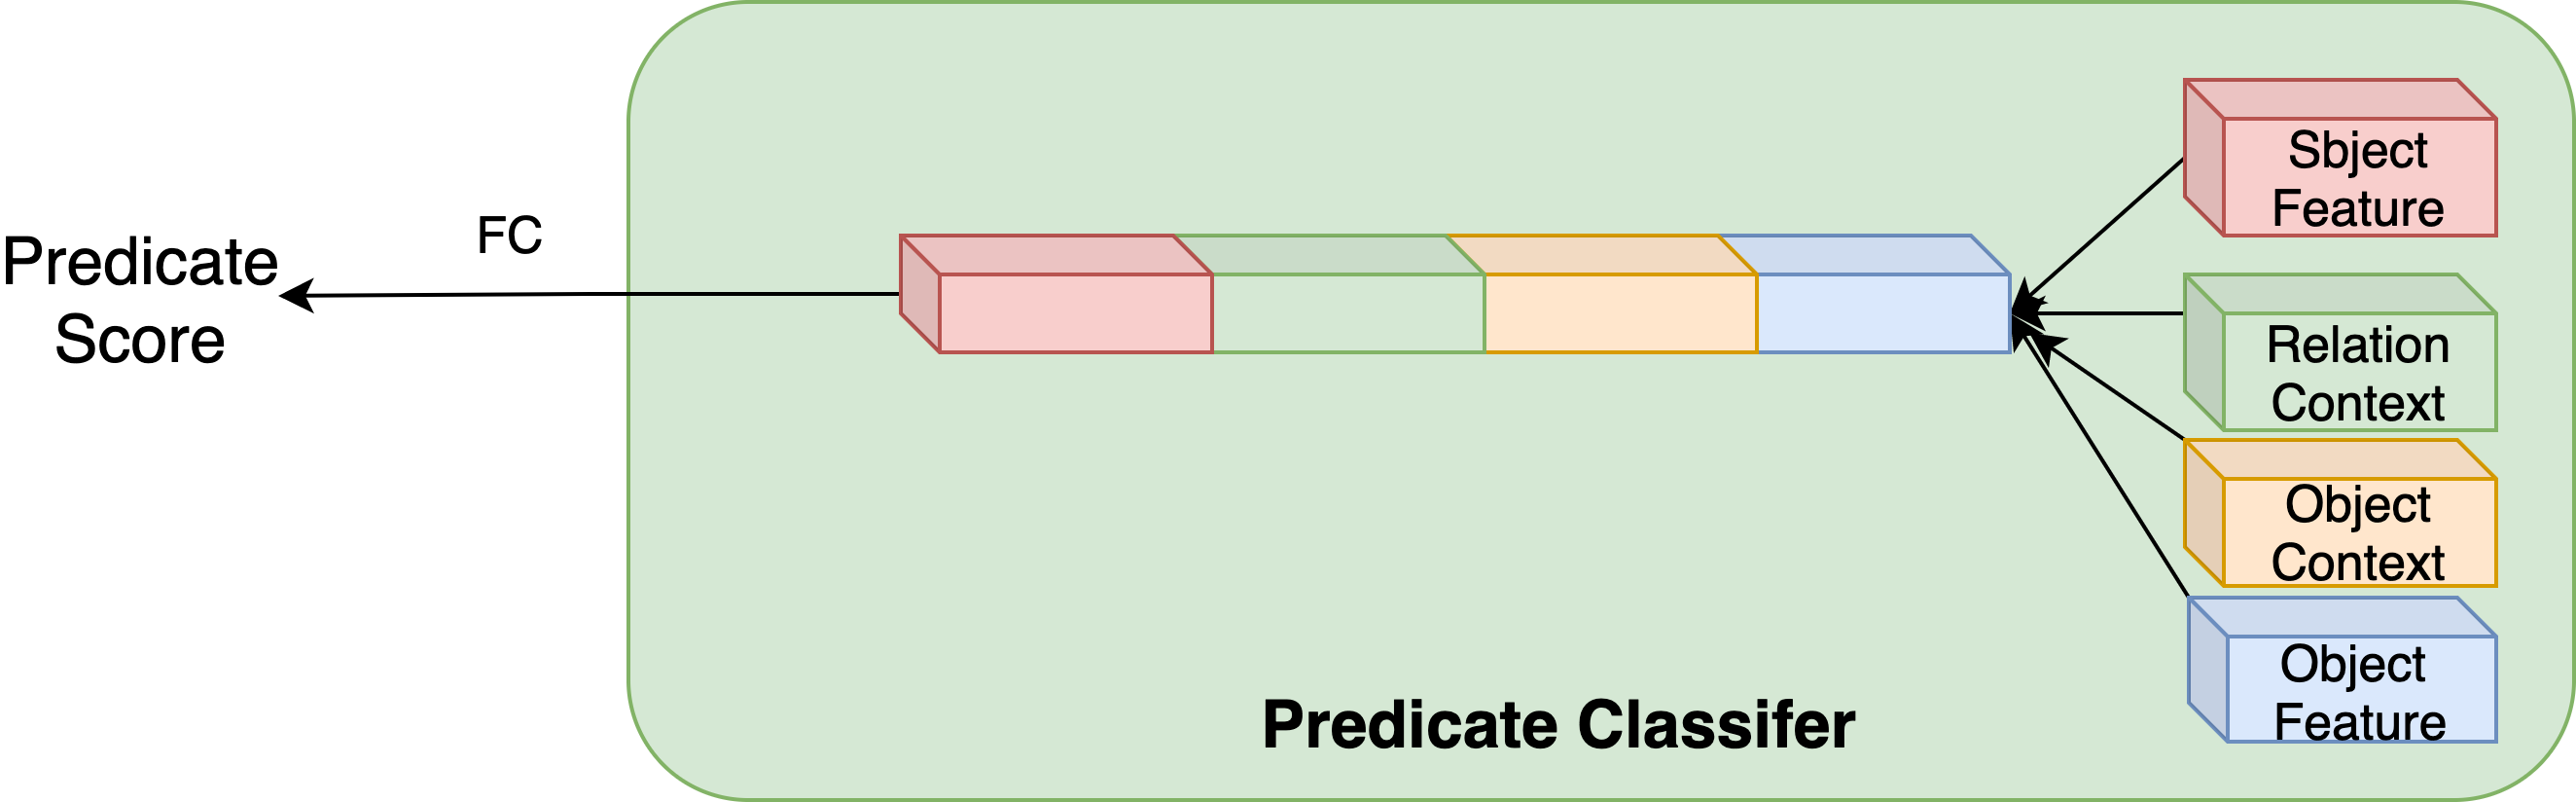
\includegraphics[width=1\linewidth]{figures/predicate_classifer}
	\caption[Illustration of the predicate classfier]{Illustration of the predicate classfier.}
	\label{fig:predicateclassifer}
\end{figure}

Predicate prediction is the last step of visual relation detection. It needs to use the previously obtained features to solve the predicate in the relation. The object features and object context have been obtained from the object decoder, and the relation context is obtained from the relation decoder. Using this information, the predicate classifier is designed to obtain the distribution of the predicate. The predicate distribution is expressed as the following Equation:%predicate 分布表示为如下的公式 

\begin{equation}
	score_{pred}(i,j) = Linear(concat(feat_{obj}^i, context_{rel}^{ij}, context_{obj}^i, feat_{obj}^j)
	\label{equ:predicatc}
\end{equation}


where $ i $ is the index of subject, $ j $ is the index of object,  $ feat_{obj} $ is the visual feature obtained from the Object Decoder, so $ feat_{obj}^i $ is the visual feature of the subject, and the $ feat_{obj}^j $ is the visual feature of the object. $ context_{rel}^{ij} $ is the relation context of the realtion $ pair(subject_i,object_j)  $obtained from the Relation Decoder, $  context_{obj}^i $ is the object context of the $subject_i$ obtained from the Object Decoder. After getting the distribution of the predicate ($score_{pred}(i,j)$), calculate the loss by Cross Entropy Loss Function with the ground truth predicate:

$$
\operatorname{loss}(\boldsymbol{x}, \text { label }=i)=-\log \left(\frac{e^{x_{i}}}{\sum_{k=1}^{N} e^{x_{k}}}\right)
$$

where $ i $ is the label of the predicate,  $ x_i $ is the score of label $ i $ in  $ score_{pred} $. Minimizing this loss in the training encourages that the probability($ x_i $) predicted by the neural network is maximal.



\subsection{Attention Loss}

In the model structure, the Object feature is based on the self attention module in the decoder structure, and the object feature is also accompanied by an attention map. The size of the attention map is 64x1369, and each row has a vector size of 1369, corresponding to an object's attention to the entire image, which can be converted into a 37x37 small attention map.The attention map is the weight of the object feature, which represents the most concerned information of the object in the image, and the position of this information should preferably correspond to the object, so that the quality of the object feature can be more intuitively evaluated. Therefore the attention loss is designed to adjust the distribution of the attention map. The scaled bounding box is applied to determine the position of the object in the attention map:

%In the object decoder(see in Fig.~\ref{fig:objectdecoder}), we obtain the object visual feature through the second Multihead Attention module, and the attention maps size of $ [64, 1369] $. We can convert it to a tensor of $ [64, 37, 37], $ which means the attention weights of each object to each pixel in the image feature from the encoder.
%As shown in Fig.~\ref{fig:attentionmap}, we get an attention weights map of size 64x1369, and each row of it can be transformed into a small attention map of 37x37 size. We hope that this attention map can have a spatial correspondence with the entity in the picture. For example, in this picture we can see a man wearing a purple jacket and two buses. We hope to find the corresponding object in the small attention map, we will find green in the attention map of the jacket. The attention weight of the part is much higher than the blue one. This shows that we pay more attention to this green area when generating the object feature of the jacket. In this way, we can better visualize the object and make our object feature better.
%Therefore, we designed an attention loss according to the ranking loss, so that the attention weights of the green area are higher than that of the blue area:

\begin{equation}
	loss_{attention}=max(0, \frac{1}{m}\sum_{m}Att_j^{no\_obj}-\frac{1}{n}\sum_{n}Att_i^{obj}+0.25
	/1369)
\end{equation}

where:
\begin{itemize}
	\item $Att_j^{no\_obj}$: the $  j^{th}  $ attention weight  of the background,
	\item $ Att_i^{obj} $ :  the $ i^{th} $ attention weight of ground truth object.
	\item Margin=0.25/1369.
	\item m:  the total number of $Att_j^{no\_obj}$.
	\item n: the total number of $ Att_i^{obj} $ .
\end{itemize}


In Figure~\ref{fig:attentionmap}, there are two buses and a man wearing a purple jacket. On the left is the original attention weights map, and its small attention map for each layer is represented as the matrix in the middle of the figure.The area in the small attention map corresponding to each object is the green part, and the blue area can be defined as the background. The purpose of this loss function is to make the attention values ($ \forall Att_i^{obj} $)  of the green area larger and the attention map ($ \forall Att_j^{no\_obj}$) ofof the blue area smaller when training the model. In this way, when processing this picture, each row in the attention map can accurately express the attention weights of the corresponding object, which makes the generated object feature more focused on the visual information of its own area.

 \begin{figure}[htp!]
	\centering
	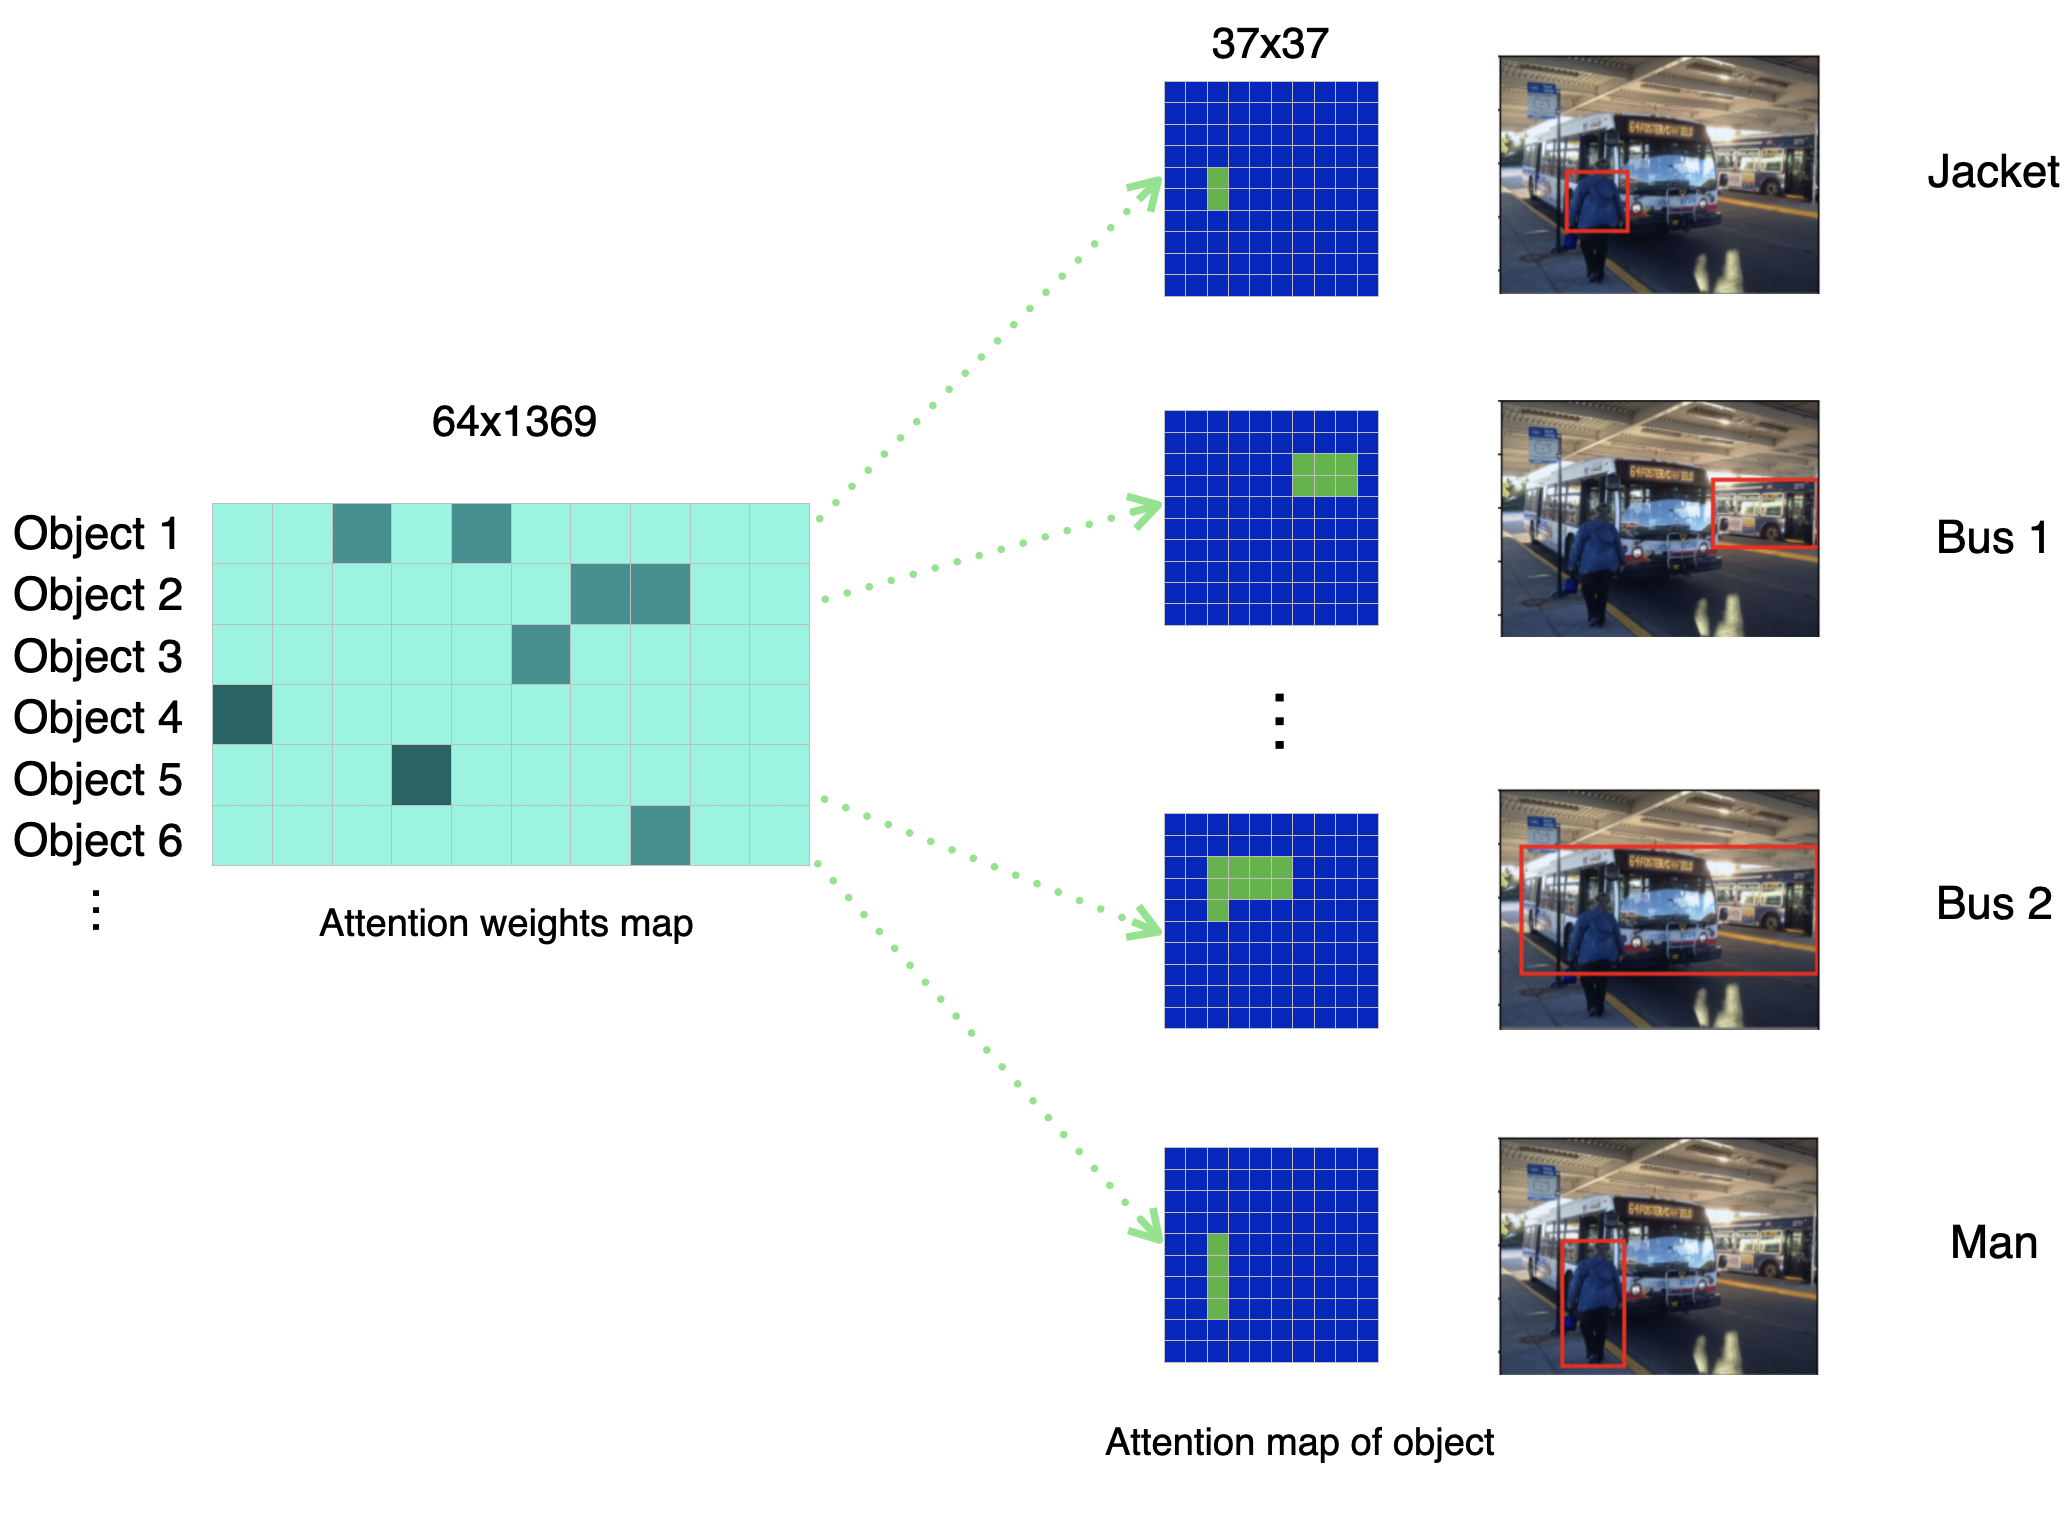
\includegraphics[width=0.9\linewidth]{figures/attention_map}
	\caption[Illustration of the attention map]{Each row in the attention weights map represents the attention of each object. }
	\label{fig:attentionmap}
\end{figure} 

This attention loss is similar to the pixel attention loss in Sec.~\ref{sec:pixelattentionloss}, both of which are adjustments to the attention map. The focus of this attention loss is the object, which makes the object feature better.

This attention loss is similar to the pixel attention loss in Sec.~\ref{sec:pixelattentionloss}, both of which are adjustments to the attention map. The focus of this attention loss is the object, which makes the object feature better. If attention loss is not used, the object decoder will pay attention to the others, In this case, the generated object feature is not well interpretable, or even wrong. In addition, the box query in PredCLS and SGCLS is defined by us, not learned through the network. The object feature queried by it may have different concerns, so its  attention weights should be restricted .% 这个attention loss 和 Sec.~\ref{sec:pixelattentionloss} 中的pixel attention loss 类似,都是对attention map的调节,这个attention loss 突出的是object ,使得object feature 更好。 如果不使用attention loss,object decoder 就会去关注它认为的需要被关注的地方,这有可能是任何地方。这样的话 ,生成的object feature 解释性就不好,甚至是错误的。还有一点,在PredCLS和SGCLS中使用的是box query,它是被我们定义的,不是通过网络学习的,由它查询出的object feature可能关注点不一样,所以我们要对它的权重(attention map)进行限制。

The total losses in the model are expressed as follows:
$$\mathcal{L} = \mathcal{L}_{pred}+\mathcal{L}_{att} +\mathcal{L}_{obj} + \mathcal{L}_{box} $$

where  $ \mathcal{L}_{pred} $ is the loss of predicate classification obtained by cross entropy loss function, $ \mathcal{L}_{att} $ is our attention loss, $ \mathcal{L}_{obj } $ is the loss of object classification, $ \mathcal{L}_{box} $ is the regression loss of the bounding box,  consists of a GIoU loss and a $l_1$ loss.

For different evaluation models, $ \mathcal{L}  $ has different expressions. The above equation is for scene graph detection.  But$ \mathcal{L}_{box} $ is not needed for scene graph classification, and only $  \mathcal{L}_{pred}$ and $\mathcal{L}_{att} $ are required for predicate classification. 
%其中\mathcal{L}_{pred} 是通过 Cross Entropy Loss Function得到的谓语的loss,\mathcal{L}_{att} 是mathcal{L}_{att} , \mathcal{L}_{obj} 是 object classifiy时需要的loss,\mathcal{L}_{box} 是bounding box的回归loss。对于不同的评估模型,\mathcal{L} 有不同的表达,上面的公式是对于sgdet的,当进行sgcls时,不需要\mathcal{L}_{box},predcls时只需要\mathcal{L}_{pred}+\mathcal{L}_{att} 。

